% =============================================================================
%  Regression Analysis for Establishing a Relation Between Weather Parameters
%  Group 19 -- Introduction to Data Analytics (IDA)
%
%  Compile from this folder (report/) with:   pdflatex main.tex   (twice)
%  All tables, figures and quoted numbers are generated by R/Project_code.R
%  (outputs/tables/*.tex, outputs/figures/*.pdf, outputs/tables/key_numbers.tex);
%  run that script first if outputs/ is empty.
% =============================================================================
\documentclass[11pt,a4paper]{article}

\usepackage[margin=2.3cm]{geometry}
\usepackage{graphicx}
\usepackage{booktabs}
\usepackage{amsmath}
\usepackage{float}
\usepackage{caption}
\usepackage{listings}
\usepackage[hidelinks]{hyperref}

\graphicspath{{../outputs/figures/}}
\captionsetup{font=small, labelfont=bf}
\setlength{\parskip}{0.45em}
\setlength{\parindent}{0pt}

% numbers computed by R/Project_code.R
% Generated by R/Project_code.R -- key numbers quoted in the report
\newcommand{\nDays}{1575}
\newcommand{\nTrainFile}{1462}
\newcommand{\nTestFile}{114}
\newcommand{\nTrainPeriod}{1461}
\newcommand{\nTestPeriod}{114}
\newcommand{\dateStart}{2013-01-01}
\newcommand{\dateEnd}{2017-04-24}
\newcommand{\nPressFixed}{10}
\newcommand{\pressMin}{990}
\newcommand{\pressMax}{1030}
\newcommand{\pressValidLow}{\ensuremath{991.38}}
\newcommand{\pressValidHigh}{\ensuremath{1023.00}}
\newcommand{\overlapInterp}{\ensuremath{1017.19}}
\newcommand{\overlapTrainP}{\ensuremath{1016.00}}
\newcommand{\nWindCapped}{33}
\newcommand{\windCap}{\ensuremath{17.61}}
\newcommand{\windMaxRaw}{\ensuremath{42.22}}
\newcommand{\nWindZthree}{14}
\newcommand{\windQone}{\ensuremath{3.70}}
\newcommand{\windQthree}{\ensuremath{9.26}}
\newcommand{\windSkewRaw}{\ensuremath{1.38}}
\newcommand{\windSkewClean}{\ensuremath{0.62}}
\newcommand{\nWindZero}{25}
\newcommand{\monsoonTemp}{\ensuremath{31.4}}
\newcommand{\monsoonHum}{\ensuremath{63}}
\newcommand{\DWmin}{\ensuremath{0.07}}
\newcommand{\DWmax}{\ensuremath{1.13}}
\newcommand{\cookMin}{\ensuremath{+0.020}}
\newcommand{\cookMax}{\ensuremath{+0.044}}
\newcommand{\nInflMin}{42}
\newcommand{\nInflMax}{80}
\newcommand{\nOverfit}{4}
\newcommand{\nSkipped}{6}
\newcommand{\hotMonth}{June}
\newcommand{\hotMonthTemp}{\ensuremath{33.7}}
\newcommand{\hotMonthPress}{\ensuremath{998.4}}
\newcommand{\coldMonth}{January}
\newcommand{\coldMonthTemp}{\ensuremath{13.8}}
\newcommand{\coldMonthPress}{\ensuremath{1018.1}}
\newcommand{\coldMonthHum}{\ensuremath{78}}
\newcommand{\dryMonth}{May}
\newcommand{\dryMonthHum}{\ensuremath{36}}
\newcommand{\pressSDraw}{\ensuremath{175.3}}
\newcommand{\pressSDclean}{\ensuremath{7.40}}
\newcommand{\cookThreshold}{\ensuremath{0.0025}}
\newcommand{\maxRhoGap}{\ensuremath{0.027}}
\newcommand{\spikeRatioMax}{\ensuremath{17}}
\newcommand{\windCapGainMin}{\ensuremath{0.015}}
\newcommand{\windCapGainMax}{\ensuremath{0.021}}
\newcommand{\nGNconv}{21}
\newcommand{\nGNtotal}{21}
\newcommand{\GNitMin}{2}
\newcommand{\GNitMax}{6}
\newcommand{\RmonthT}{\ensuremath{87}}
\newcommand{\acfT}{\ensuremath{0.97}}
\newcommand{\RmonthH}{\ensuremath{58}}
\newcommand{\acfH}{\ensuremath{0.88}}
\newcommand{\RmonthW}{\ensuremath{17}}
\newcommand{\acfW}{\ensuremath{0.50}}
\newcommand{\RmonthP}{\ensuremath{88}}
\newcommand{\acfP}{\ensuremath{0.97}}
\newcommand{\rTH}{\ensuremath{-0.574}}
\newcommand{\rhoTH}{\ensuremath{-0.578}}
\newcommand{\rCIloTH}{\ensuremath{-0.606}}
\newcommand{\rCIhiTH}{\ensuremath{-0.539}}
\newcommand{\neffTH}{\ensuremath{118}}
\newcommand{\RlinTH}{\ensuremath{0.329}}
\newcommand{\RlinTestTH}{\ensuremath{0.122}}
\newcommand{\RlinTrainTH}{\ensuremath{0.325}}
\newcommand{\interceptTH}{\ensuremath{40.23}}
\newcommand{\slopeTH}{\ensuremath{-0.2482}}
\newcommand{\slopeCIloTH}{\ensuremath{-0.2657}}
\newcommand{\slopeCIhiTH}{\ensuremath{-0.2307}}
\newcommand{\slopeRevTH}{\ensuremath{-1.3254}}
\newcommand{\DWTH}{\ensuremath{0.07}}
\newcommand{\bestTH}{cubic}
\newcommand{\RbestTH}{\ensuremath{0.331}}
\newcommand{\RbestTestTH}{\ensuremath{0.132}}
\newcommand{\bestNLTH}{cubic}
\newcommand{\gainTH}{\ensuremath{+0.002}}
\newcommand{\RbestNLTestTH}{\ensuremath{0.132}}
\newcommand{\maxGainTH}{\ensuremath{+0.002}}
\newcommand{\maxGainCurveTH}{cubic}
\newcommand{\ranomTH}{\ensuremath{-0.550}}
\newcommand{\RanomTH}{\ensuremath{0.302}}
\newcommand{\seasShareTH}{\ensuremath{8}}
\newcommand{\rWinterTH}{\ensuremath{-0.47}}
\newcommand{\rSummerTH}{\ensuremath{-0.81}}
\newcommand{\rMonsoonTH}{\ensuremath{-0.80}}
\newcommand{\rPostTH}{\ensuremath{-0.16}}
\newcommand{\cookChangeTH}{\ensuremath{+0.031}}
\newcommand{\nInflTH}{42}
\newcommand{\rTW}{\ensuremath{0.313}}
\newcommand{\rhoTW}{\ensuremath{0.340}}
\newcommand{\rCIloTW}{\ensuremath{0.268}}
\newcommand{\rCIhiTW}{\ensuremath{0.357}}
\newcommand{\neffTW}{\ensuremath{543}}
\newcommand{\RlinTW}{\ensuremath{0.098}}
\newcommand{\RlinTestTW}{\ensuremath{-0.502}}
\newcommand{\RlinTrainTW}{\ensuremath{0.113}}
\newcommand{\interceptTW}{\ensuremath{21.45}}
\newcommand{\slopeTW}{\ensuremath{0.5548}}
\newcommand{\slopeCIloTW}{\ensuremath{0.4716}}
\newcommand{\slopeCIhiTW}{\ensuremath{0.6380}}
\newcommand{\slopeRevTW}{\ensuremath{0.1768}}
\newcommand{\DWTW}{\ensuremath{0.16}}
\newcommand{\bestTW}{exponential}
\newcommand{\RbestTW}{\ensuremath{0.094}}
\newcommand{\RbestTestTW}{\ensuremath{-0.479}}
\newcommand{\bestNLTW}{exponential}
\newcommand{\gainTW}{\ensuremath{-0.004}}
\newcommand{\RbestNLTestTW}{\ensuremath{-0.479}}
\newcommand{\maxGainTW}{\ensuremath{+0.013}}
\newcommand{\maxGainCurveTW}{cubic}
\newcommand{\ranomTW}{\ensuremath{0.137}}
\newcommand{\RanomTW}{\ensuremath{0.019}}
\newcommand{\seasShareTW}{\ensuremath{81}}
\newcommand{\rWinterTW}{\ensuremath{0.19}}
\newcommand{\rSummerTW}{\ensuremath{0.14}}
\newcommand{\rMonsoonTW}{\ensuremath{0.30}}
\newcommand{\rPostTW}{\ensuremath{0.22}}
\newcommand{\cookChangeTW}{\ensuremath{+0.043}}
\newcommand{\nInflTW}{44}
\newcommand{\RrawWindTW}{\ensuremath{0.082}}
\newcommand{\rTP}{\ensuremath{-0.881}}
\newcommand{\rhoTP}{\ensuremath{-0.881}}
\newcommand{\rCIloTP}{\ensuremath{-0.891}}
\newcommand{\rCIhiTP}{\ensuremath{-0.869}}
\newcommand{\neffTP}{\ensuremath{41}}
\newcommand{\RlinTP}{\ensuremath{0.776}}
\newcommand{\RlinTestTP}{\ensuremath{0.755}}
\newcommand{\RlinTrainTP}{\ensuremath{0.773}}
\newcommand{\interceptTP}{\ensuremath{905.61}}
\newcommand{\slopeTP}{\ensuremath{-0.8729}}
\newcommand{\slopeCIloTP}{\ensuremath{-0.8961}}
\newcommand{\slopeCIhiTP}{\ensuremath{-0.8497}}
\newcommand{\slopeRevTP}{\ensuremath{-0.8889}}
\newcommand{\DWTP}{\ensuremath{0.28}}
\newcommand{\bestTP}{cubic}
\newcommand{\RbestTP}{\ensuremath{0.819}}
\newcommand{\RbestTestTP}{\ensuremath{0.715}}
\newcommand{\bestNLTP}{cubic}
\newcommand{\gainTP}{\ensuremath{+0.043}}
\newcommand{\RbestNLTestTP}{\ensuremath{0.715}}
\newcommand{\maxGainTP}{\ensuremath{+0.043}}
\newcommand{\maxGainCurveTP}{cubic}
\newcommand{\ranomTP}{\ensuremath{-0.431}}
\newcommand{\RanomTP}{\ensuremath{0.186}}
\newcommand{\seasShareTP}{\ensuremath{76}}
\newcommand{\rWinterTP}{\ensuremath{-0.51}}
\newcommand{\rSummerTP}{\ensuremath{-0.86}}
\newcommand{\rMonsoonTP}{\ensuremath{-0.31}}
\newcommand{\rPostTP}{\ensuremath{-0.77}}
\newcommand{\cookChangeTP}{\ensuremath{+0.031}}
\newcommand{\nInflTP}{69}
\newcommand{\rHW}{\ensuremath{-0.400}}
\newcommand{\rhoHW}{\ensuremath{-0.413}}
\newcommand{\rCIloHW}{\ensuremath{-0.441}}
\newcommand{\rCIhiHW}{\ensuremath{-0.358}}
\newcommand{\neffHW}{\ensuremath{609}}
\newcommand{\RlinHW}{\ensuremath{0.160}}
\newcommand{\RlinTestHW}{\ensuremath{0.099}}
\newcommand{\RlinTrainHW}{\ensuremath{0.162}}
\newcommand{\interceptHW}{\ensuremath{71.57}}
\newcommand{\slopeHW}{\ensuremath{-1.6379}}
\newcommand{\slopeCIloHW}{\ensuremath{-1.8234}}
\newcommand{\slopeCIhiHW}{\ensuremath{-1.4523}}
\newcommand{\slopeRevHW}{\ensuremath{-0.0977}}
\newcommand{\DWHW}{\ensuremath{0.37}}
\newcommand{\bestHW}{exponential}
\newcommand{\RbestHW}{\ensuremath{0.165}}
\newcommand{\RbestTestHW}{\ensuremath{0.097}}
\newcommand{\bestNLHW}{exponential}
\newcommand{\gainHW}{\ensuremath{+0.005}}
\newcommand{\RbestNLTestHW}{\ensuremath{0.097}}
\newcommand{\maxGainHW}{\ensuremath{+0.011}}
\newcommand{\maxGainCurveHW}{cubic}
\newcommand{\ranomHW}{\ensuremath{-0.315}}
\newcommand{\RanomHW}{\ensuremath{0.100}}
\newcommand{\seasShareHW}{\ensuremath{38}}
\newcommand{\rWinterHW}{\ensuremath{-0.31}}
\newcommand{\rSummerHW}{\ensuremath{-0.25}}
\newcommand{\rMonsoonHW}{\ensuremath{-0.40}}
\newcommand{\rPostHW}{\ensuremath{-0.47}}
\newcommand{\cookChangeHW}{\ensuremath{+0.020}}
\newcommand{\nInflHW}{67}
\newcommand{\RrawWindHW}{\ensuremath{0.139}}
\newcommand{\rHP}{\ensuremath{0.339}}
\newcommand{\rhoHP}{\ensuremath{0.332}}
\newcommand{\rCIloHP}{\ensuremath{0.295}}
\newcommand{\rCIhiHP}{\ensuremath{0.382}}
\newcommand{\neffHP}{\ensuremath{118}}
\newcommand{\RlinHP}{\ensuremath{0.115}}
\newcommand{\RlinTestHP}{\ensuremath{0.133}}
\newcommand{\RlinTrainHP}{\ensuremath{0.107}}
\newcommand{\interceptHP}{\ensuremath{-722.90}}
\newcommand{\slopeHP}{\ensuremath{0.7767}}
\newcommand{\slopeCIloHP}{\ensuremath{0.6701}}
\newcommand{\slopeCIhiHP}{\ensuremath{0.8832}}
\newcommand{\slopeRevHP}{\ensuremath{0.1481}}
\newcommand{\DWHP}{\ensuremath{0.26}}
\newcommand{\bestHP}{quadratic}
\newcommand{\RbestHP}{\ensuremath{0.187}}
\newcommand{\RbestTestHP}{\ensuremath{0.292}}
\newcommand{\bestNLHP}{quadratic}
\newcommand{\gainHP}{\ensuremath{+0.072}}
\newcommand{\RbestNLTestHP}{\ensuremath{0.292}}
\newcommand{\maxGainHP}{\ensuremath{+0.072}}
\newcommand{\maxGainCurveHP}{cubic}
\newcommand{\ranomHP}{\ensuremath{0.157}}
\newcommand{\RanomHP}{\ensuremath{0.025}}
\newcommand{\seasShareHP}{\ensuremath{78}}
\newcommand{\rWinterHP}{\ensuremath{0.19}}
\newcommand{\rSummerHP}{\ensuremath{0.70}}
\newcommand{\rMonsoonHP}{\ensuremath{0.01}}
\newcommand{\rPostHP}{\ensuremath{0.07}}
\newcommand{\cookChangeHP}{\ensuremath{+0.044}}
\newcommand{\nInflHP}{80}
\newcommand{\rWP}{\ensuremath{-0.299}}
\newcommand{\rhoWP}{\ensuremath{-0.315}}
\newcommand{\rCIloWP}{\ensuremath{-0.344}}
\newcommand{\rCIhiWP}{\ensuremath{-0.254}}
\newcommand{\neffWP}{\ensuremath{542}}
\newcommand{\RlinWP}{\ensuremath{0.090}}
\newcommand{\RlinTestWP}{\ensuremath{-0.356}}
\newcommand{\RlinTrainWP}{\ensuremath{0.105}}
\newcommand{\interceptWP}{\ensuremath{175.66}}
\newcommand{\slopeWP}{\ensuremath{-0.1674}}
\newcommand{\slopeCIloWP}{\ensuremath{-0.1938}}
\newcommand{\slopeCIhiWP}{\ensuremath{-0.1410}}
\newcommand{\slopeRevWP}{\ensuremath{-0.5350}}
\newcommand{\DWWP}{\ensuremath{1.09}}
\newcommand{\bestWP}{cubic}
\newcommand{\RbestWP}{\ensuremath{0.091}}
\newcommand{\RbestTestWP}{\ensuremath{-0.351}}
\newcommand{\bestNLWP}{cubic}
\newcommand{\gainWP}{\ensuremath{+0.001}}
\newcommand{\RbestNLTestWP}{\ensuremath{-0.351}}
\newcommand{\maxGainWP}{\ensuremath{+0.001}}
\newcommand{\maxGainCurveWP}{cubic}
\newcommand{\ranomWP}{\ensuremath{-0.104}}
\newcommand{\RanomWP}{\ensuremath{0.011}}
\newcommand{\seasShareWP}{\ensuremath{88}}
\newcommand{\rWinterWP}{\ensuremath{-0.10}}
\newcommand{\rSummerWP}{\ensuremath{-0.17}}
\newcommand{\rMonsoonWP}{\ensuremath{-0.16}}
\newcommand{\rPostWP}{\ensuremath{-0.21}}
\newcommand{\cookChangeWP}{\ensuremath{+0.028}}
\newcommand{\nInflWP}{66}
\newcommand{\RrawWindWP}{\ensuremath{0.074}}
\newcommand{\cubicPeakTP}{\ensuremath{998.0}}
\newcommand{\lineRankFirst}{215}
\newcommand{\lineRankLast}{231}
\newcommand{\linePearsonFirst}{233}
\newcommand{\linePearsonLast}{245}
\newcommand{\lineSlrFirst}{1300}
\newcommand{\lineSlrLast}{1347}
\newcommand{\lineSolveFirst}{351}
\newcommand{\lineSolveLast}{390}
\newcommand{\lineGaussNewtonFirst}{393}
\newcommand{\lineGaussNewtonLast}{442}
\newcommand{\linePolyFirst}{1625}
\newcommand{\linePolyLast}{1644}
\newcommand{\lineExpFirst}{1646}
\newcommand{\lineExpLast}{1678}


\newcommand{\submissiondate}{7 October 2026}   % <-- set the actual submission date
\newcommand{\var}[1]{\texttt{#1}}
\newcommand{\Rsq}{R^2}
\newcommand{\tabinput}[1]{\input{../outputs/tables/#1}}

\lstset{
  language=R, basicstyle=\ttfamily\scriptsize, columns=fullflexible,
  keepspaces=true, breaklines=true, frame=single, numbers=left,
  numberstyle=\tiny, numberfirstline=true, showstringspaces=false,
  commentstyle=\itshape, keywordstyle=\ttfamily
}

\begin{document}

% ---------------------------------------------------------------- front page
\begin{titlepage}
  \centering
  \vspace*{2cm}
  {\LARGE\bfseries Regression Analysis for Establishing a Relation\\[0.3em]
   Between Weather Parameters\par}
  \vspace{1.2cm}
  {\large Project Report\par}
  \vspace{0.4cm}
  {\large Course: Introduction to Data Analytics (IDA)\par}
  \vspace{0.3cm}
  {\large Group ID: 19\par}
  \vspace{1.5cm}

  {\large\bfseries Team members\par}
  \vspace{0.3cm}
  {\small
  \begin{tabular}{llll}
    \toprule
    Name & Roll No. & Email & Programme \\
    \midrule
    Aditya Palapati (group leader) & S20230010176 & \texttt{aditya.p23@iiits.in}      & UG4, CSE \\
    Meghana Kuruva                 & S20230010134 & \texttt{meghana.k23@iiits.in}     & UG4, CSE \\
    Rohin Sai Bogadi               & S20230010047 & \texttt{rohinsai.b23@iiits.in}    & UG4, CSE \\
    Srimeenakshi K S               & S20262010002 & \texttt{srimeenakshi.ks@iiits.in} & PhD (full time), CSE \\
    \bottomrule
  \end{tabular}}

  \vfill
  {\large Date of submission: \submissiondate\par}
\end{titlepage}

% ---------------------------------------------------------------- abstract
\begin{abstract}
We analyse \nDays{} consecutive days (\dateStart{} to \dateEnd) of the Daily Delhi
Climate data to establish how mean temperature, humidity, wind speed and mean
pressure are related. After repairing \nPressFixed{} physically impossible pressure
values and capping \nWindCapped{} implausible wind speeds, we fit, for every one of
the six pairs of parameters, a simple linear model and five simple non-linear
models (quadratic, cubic, exponential, logarithmic, power). Every estimator,
including least squares, Gauss--Newton and the normal equations, is implemented
from scratch in base R. Temperature and pressure are by far the most strongly
related parameters ($r=\rTP$, linear $\Rsq=\RlinTP$, cubic $\Rsq=\RbestTP$),
followed by temperature and humidity ($\Rsq=\RlinTH$); the four relations
involving wind speed or humidity--pressure explain less than 20\% of the variance.
A non-linear curve improves the fit meaningfully ($\Delta\Rsq>0.05$) for one relation
only, humidity--pressure ($\Delta\Rsq=\gainHP$). Removing the annual cycle shows
that \seasShareTP\% of the temperature--pressure $\Rsq$ is shared seasonality,
whereas the temperature--humidity relation is a genuine day-to-day relation
(only \seasShareTH\% seasonal).
\end{abstract}

\tableofcontents
\clearpage

% ---------------------------------------------------------------- 3
\section{Introduction and problem statement}

A first look at the Delhi data already suggests that the four parameters move
together. Averaged over 2013--2017, \hotMonth{} is the hottest month
(\hotMonthTemp\,$^\circ$C) and also has one of the lowest mean pressures
(\hotMonthPress\,hPa), while \coldMonth{} is the coldest (\coldMonthTemp\,$^\circ$C) with
the highest pressure (\coldMonthPress\,hPa) and a humidity of \coldMonthHum\%; the driest
month is \dryMonth{} with only \dryMonthHum\% humidity. Our task was to turn such
impressions into measured relations. The assignment asks us to
\begin{enumerate}
  \item[(a)] pre-process the data properly,
  \item[(b)] find the relation between each pair of weather parameters,
  \item[(c)] report the relation using (i) simple linear regression and
             (ii) simple non-linear regression, and
  \item[(d)] calculate $\Rsq$ for every case and conclude precisely.
\end{enumerate}
With four parameters there are six pairs. ``Simple'' regression means one
predictor per model, so each relation is studied as $y=f(x)$ for a single pair
$(x,y)$. Because a regression of $y$ on $x$ is not the same as a regression of
$x$ on $y$, we fix a primary direction for each pair (Section~\ref{sec:lin}) and
also report the reverse direction.

Two properties of the data shape the whole analysis and are discussed
throughout: the observations form a \emph{daily time series} (consecutive days
are strongly correlated), and all four parameters follow a pronounced
\emph{annual cycle}. A high $\Rsq$ between two seasonal variables can therefore
reflect their shared seasonality rather than a direct link, and we test this
explicitly in Section~\ref{sec:r2}.

% ---------------------------------------------------------------- 4
\section{Dataset description}

We use the \emph{Daily Delhi Climate} dataset~\cite{kaggle}: daily averages of four
weather measurements in New Delhi (Table~\ref{tab:vars}), delivered as two files:
\begin{itemize}
  \item \texttt{DailyDelhiClimateTrain.csv}: \nTrainFile{} days, 2013-01-01 to 2017-01-01;
  \item \texttt{DailyDelhiClimateTest.csv}: \nTestFile{} days, 2017-01-01 to 2017-04-24.
\end{itemize}

\begin{table}[htbp]
  \centering
  \caption{Variables of the dataset. Units were verified from the observed ranges
           (e.g.\ a mean wind speed of about 7 corresponds to 1.9\,m/s if read as km/h,
           which is typical for Delhi; read as m/s it would be implausibly windy every day).}
  \label{tab:vars}
  \begin{tabular}{lll}
    \toprule
    Variable & Meaning & Unit \\
    \midrule
    \var{date}         & calendar day                        & -- \\
    \var{meantemp}     & mean temperature of the day         & $^\circ$C \\
    \var{humidity}     & mean relative humidity              & \% \\
    \var{wind\_speed}  & mean wind speed                     & km/h \\
    \var{meanpressure} & mean (sea-level) atmospheric pressure & hPa \\
    \bottomrule
  \end{tabular}
\end{table}

\paragraph{Data-quality issues.} The raw files contain no missing values and no
duplicate dates within a file, but:
\begin{itemize}
  \item \textbf{Mean pressure} has \nPressFixed{} physically impossible values, e.g.\
        7679.33, 1352.62, $-3.04$ and 12.05\,hPa in the training file and 59.0\,hPa on
        2017-01-01 in the test file. All credible values lie between \pressValidLow{}
        and \pressValidHigh{}\,hPa, and the days around each bad value are normal, so
        these are recording errors, not weather.
  \item \textbf{Wind speed} has isolated extreme daily means up to \windMaxRaw\,km/h, against a
        third quartile of \windQthree\,km/h.
  \item \textbf{Overlap}: 2017-01-01 appears in both files with different values.
\end{itemize}

Descriptive statistics of the cleaned data are given in Table~\ref{tab:descriptive_stats}
and their distributions in Figure~\ref{fig:hist}. Temperature and pressure are
bimodal (a cool high-pressure and a hot low-pressure regime), humidity is
slightly left-skewed and wind speed is right-skewed.

\tabinput{descriptive_stats}

\begin{figure}[htbp]
  \centering
  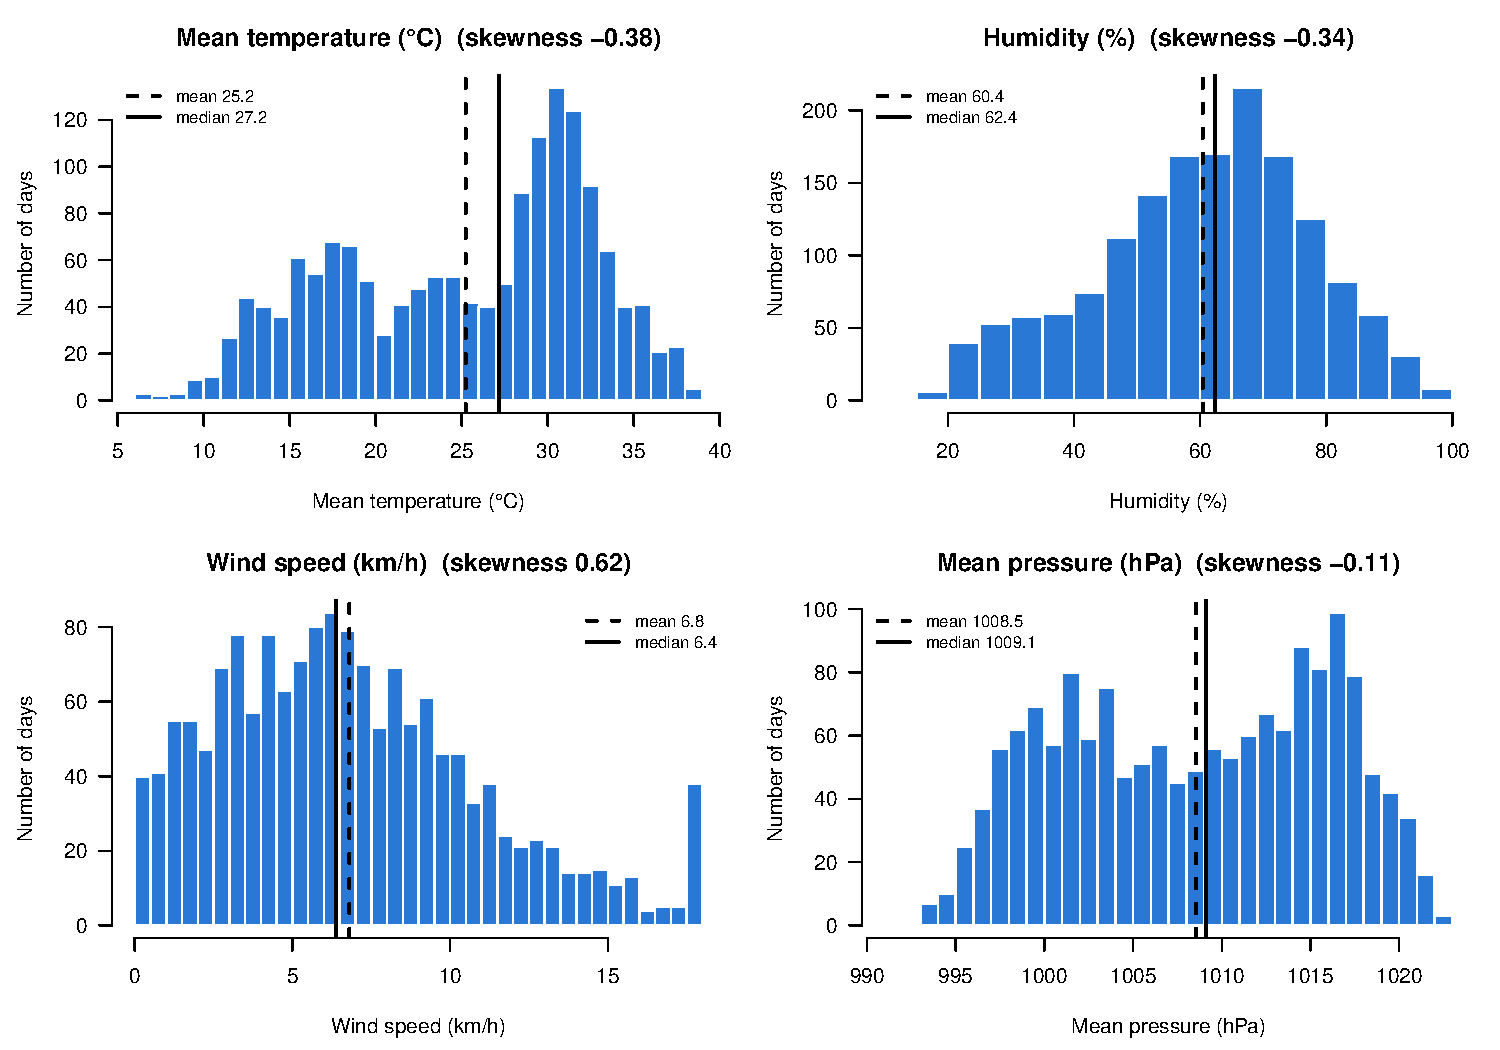
\includegraphics[width=0.9\linewidth]{histograms.pdf}
  \caption{Histograms of the cleaned daily data with mean (dashed) and median (solid).}
  \label{fig:hist}
\end{figure}

% ---------------------------------------------------------------- 5
\section{Methodology}
\label{sec:method}

All computations were implemented in \textbf{base R without any external
package}. We did not use any ready-made statistics or modelling function
(\texttt{lm}, \texttt{nls}, \texttt{cor}, \texttt{var}, \texttt{sd},
\texttt{quantile}, \texttt{median}, \texttt{approx}, \texttt{solve}, \dots); the
only built-in statistical function used is \texttt{pt()}, the cumulative
distribution function of Student's $t$, for $p$-values. The submitted script
\texttt{R/Project\_code.R} contains every formula below as a commented function.
For our own checking only, we compared all results with R's built-in functions:
correlations, linear and polynomial fits agree to better than $10^{-11}$, and the
Gauss--Newton fits agree with \texttt{nls} to within its convergence tolerance.

\subsection{Descriptive statistics and correlation}
The summary tables are produced by our own mean, variance ($n-1$ divisor),
type-7 quantile~\cite{hyndman} and skewness functions. Skewness,
$G_1=\frac{\sqrt{n(n-1)}}{n-2}\,m_3/m_2^{3/2}$ with $m_k=\frac1n\sum(x_i-\bar x)^k$, was
the number that told us how much the wind-speed outliers distorted that variable
(\windSkewRaw{} before and \windSkewClean{} after capping).

For each pair we computed the Pearson coefficient from the centred cross-products,
\[
  r=\frac{S_{xy}}{\sqrt{S_{xx}S_{yy}}},\qquad
  S_{xy}=\sum_{i=1}^n (x_i-\bar x)(y_i-\bar y),\quad
  S_{xx}=\sum_{i=1}^n (x_i-\bar x)^2 ,
\]
and, as a check for curvature, Spearman's $\rho$~\cite{spearman}: we rank both
variables (ties share the average rank, which matters here because \nWindZero{}
days have zero wind and \nWindCapped{} days share the capped value) and apply the
same formula to the ranks. A curved but monotonic relation would make $\rho$ and
$r$ differ; we would have flagged a gap above 0.10, and the largest gap we found
was \maxRhoGap.

With $n=\nDays$, the usual test statistic $t=r\sqrt{(n-2)/(1-r^2)}$ (on $n-2$
degrees of freedom) makes every correlation in our data ``significant'', so we
report it mainly for completeness, together with a 95\% interval from Fisher's transformation~\cite{fisher}
\[
  z=\tfrac12\ln\frac{1+r}{1-r},\qquad \mathrm{SE}(z)=\frac{1}{\sqrt{n-3}},\qquad
  r\in\left[\tanh(z-1.96\,\mathrm{SE}),\ \tanh(z+1.96\,\mathrm{SE})\right].
\]
The critical value 1.96 is hard-coded because the assignment rules out \texttt{qnorm}.

The more important question for daily weather is how many \emph{independent}
observations we really have. Temperature on one day almost repeats the previous day
(lag-1 autocorrelation \acfT, pressure \acfP). Following~\cite{bartlett,bretherton} we
therefore also use the effective sample size
$n_{\mathrm{eff}}=n\,\frac{1-a_x a_y}{1+a_x a_y}$, where $a_x,a_y$ are the lag-1
autocorrelations of the two variables; for temperature and pressure it shrinks the
\nDays{} days to about \neffTP.

\subsection{Simple linear regression}
One function, \texttt{my\_slr}, fits all twelve straight lines (six pairs, two
directions). Setting the derivatives of $\sum(y_i-a-bx_i)^2$ to zero gives the
closed-form estimates we implemented~\cite{montgomery}
\[
  b=\frac{S_{xy}}{S_{xx}},\qquad a=\bar y-b\,\bar x,\qquad e_i=y_i-(a+b\,x_i).
\]
From the residuals we obtain $\mathrm{SSE}=\sum e_i^2$, and with
$\mathrm{SST}=\sum(y_i-\bar y)^2$ the two fit measures used throughout the report,
\[
  \Rsq = 1-\frac{\mathrm{SSE}}{\mathrm{SST}},\qquad
  \Rsq_{\mathrm{adj}} = 1-(1-\Rsq)\frac{n-1}{n-p-1},
\]
where $p$ counts the predictor terms (1 for a line, 3 for a cubic). For a single
line and $n=\nDays$ the adjustment is negligible; it starts to matter only when the
polynomials are compared in Section~\ref{sec:nl}. The function also returns RMSE and
MAE (in the units of $y$), the residual standard error $s=\sqrt{\mathrm{SSE}/(n-2)}$,
$\mathrm{SE}(b)=s/\sqrt{S_{xx}}$, the $t$-value of the slope and its 95\% interval
$b\pm t_{0.975,n-2}\,\mathrm{SE}(b)$. Because \texttt{qt} is not allowed, we find
$t_{0.975,n-2}$ by bisection on \texttt{pt()}; with infinite degrees of freedom the
same routine gives the normal quantiles for our Q--Q plots.

Since the rows are consecutive days, we also summarise the residuals in time order
with the Durbin--Watson statistic~\cite{durbin},
\[
  \mathrm{DW}=\frac{\sum_{t=2}^{n}(e_t-e_{t-1})^2}{\sum_{t=1}^{n}e_t^2}\approx 2(1-\hat\rho_1),
\]
which is close to 2 for independent residuals and close to 0 when each residual
repeats the previous one. Finally, to see whether a handful of days drives a fit, we
computed Cook's distance~\cite{cook}
$D_i=\frac{e_i^2}{2s^2}\,\frac{h_i}{(1-h_i)^2}$ with leverage
$h_i=\frac1n+(x_i-\bar x)^2/S_{xx}$ and refitted each line without the days above
$4/n=\cookThreshold$.

\subsection{Simple non-linear regression}
\label{sec:method-nl}
Five curves with one predictor were fitted:
\[
\begin{array}{lll}
  \text{quadratic}   & y=c_0+c_1u+c_2u^2 & \\
  \text{cubic}       & y=c_0+c_1u+c_2u^2+c_3u^3 & u=(x-\bar x)/s_x\\
  \text{exponential} & y=a\,e^{bx} & \\
  \text{logarithmic} & y=a+b\ln x & x>0\\
  \text{power}       & y=a\,x^{b} & x>0
\end{array}
\]

\textbf{Polynomials} are linear in their coefficients. With the design matrix
$X=[\mathbf 1,u,u^2(,u^3)]$ the least-squares estimate solves the normal equations
\[
  (X^\top X)\,\boldsymbol\beta = X^\top \mathbf y ,
\]
which we solve with our own Gaussian elimination with partial pivoting. The
predictor is standardised first: with raw pressures around 1000\,hPa the columns
of $X$ would be of order $1,10^3,10^6,10^9$ and $X^\top X$ numerically singular.

\textbf{Logarithmic} model: linear regression of $y$ on $\ln x$.

\textbf{Exponential and power} models are non-linear in $b$. Start values come
from linearising ($\ln y=\ln a+bx$, respectively $\ln y=\ln a+b\ln x$) and fitting
by least squares; they are then refined on the \emph{original} scale by
Gauss--Newton~\cite{bates}. With residuals $\mathbf r=\mathbf y-f(\mathbf x;\boldsymbol\theta)$
and Jacobian $J_{ij}=\partial f(x_i;\boldsymbol\theta)/\partial\theta_j$, each step solves
\[
  (J^\top J)\,\boldsymbol\delta = J^\top \mathbf r ,\qquad
  \boldsymbol\theta \leftarrow \boldsymbol\theta+\lambda\boldsymbol\delta ,
\]
with step halving ($\lambda=1,\tfrac12,\tfrac14,\dots$) until the SSE decreases.
Iteration stops when the relative decrease of the SSE or the relative step is
below $10^{-10}$ (at most 200 iterations); failures are caught and reported, not
fatal. For numerical stability the models are fitted in the equivalent centred
forms $y=A\,e^{b(x-c)}$ and $y=A\,(x/c)^b$ and converted back to $a$ and $b$. For
the exponential model the Jacobian is
$\partial f/\partial A=e^{b(x-c)}$, $\partial f/\partial b=A(x-c)e^{b(x-c)}$.

\textbf{$\Rsq$ on the original scale.} For \emph{every} model,
$\Rsq=1-\mathrm{SSE}/\mathrm{SST}$ is computed from the residuals of $y$ itself (not
of $\ln y$), so all curves are compared on the same footing. Models that are
mathematically undefined are skipped and recorded: $\ln x$ does not exist for the
\nWindZero{} days with zero wind speed, so the logarithmic and power models with
wind speed as predictor were not fitted.

\subsection{Model evaluation and selection}
\label{sec:selection}
The headline numbers are full-data fits. As an out-of-sample check every model
is also fitted on 2013--2016 (\nTrainPeriod{} days) and evaluated on 2017
(\nTestPeriod{} days, January--April):
$\Rsq_{\text{test}}=1-\sum(y_t-\hat y_t)^2/\sum(y_t-\bar y_{\text{test}})^2$ with
$\hat y_t$ from the training coefficients. To avoid rewarding a polynomial merely
for its extra parameters, the curve selected for each relation maximises
\[
  \text{score}=\tfrac12\left(\Rsq_{\mathrm{adj}}+\Rsq_{\text{test}}\right).
\]
An improvement over the line is called \emph{meaningful} if
$\Delta\Rsq=\Rsq_{\text{best non-linear}}-\Rsq_{\text{linear}}>0.05$.

\subsection{Seasonality}
To separate shared seasonality from day-to-day association we compute
\emph{anomalies} $\tilde x_t=x_t-\bar x_{m(t)}$, where $\bar x_{m}$ is the mean of
calendar month $m$ over all years, and correlate the anomalies. The share of the
$\Rsq$ that disappears, $1-r_{\text{anom}}^2/r^2$, is the part explained by the
common annual cycle. Seasons follow the India Meteorological Department
convention: winter (Dec--Feb), summer/pre-monsoon (Mar--May), monsoon (Jun--Sep)
and post-monsoon (Oct--Nov).

% ---------------------------------------------------------------- 6
\section{Data pre-processing (2a)}
\label{sec:prep}

The steps below are performed in Section~2 of the script; Table~\ref{tab:preprocessing_summary}
counts the rows and values affected and Figures~\ref{fig:box}--\ref{fig:ts} show
the effect.

\begin{enumerate}
  \item \textbf{Combine and sort.} Both files are bound into one data frame with a
        \var{source} column, dates are parsed and the rows sorted by date.
  \item \textbf{Overlapping date.} 2017-01-01 occurs in both files. The training row
        (10.0\,$^\circ$C, 100\% humidity, 0.0\,km/h, 1016\,hPa) consists of round numbers
        with saturated humidity and no wind, i.e.\ a single reading rather than a daily
        mean; the test row holds proper daily averages but an invalid pressure. We keep
        the test row and drop the training row, leaving \nDays{} days.
  \item \textbf{Date continuity.} The days from \dateStart{} to \dateEnd{} form a complete
        daily sequence: no missing and no duplicate dates.
  \item \textbf{Range checks.} Humidity lies within 0--100\% and no wind speed is negative.
        The \nWindZero{} days with zero wind are kept: calm days are physically possible.
  \item \textbf{Invalid pressure.} The \nPressFixed{} values outside
        \pressMin--\pressMax\,hPa are set to missing and filled by linear interpolation
        in time between the neighbouring valid days. Pressure changes smoothly from day to
        day (lag-1 autocorrelation \acfP), so interpolation is accurate, and the other three
        variables of those days are kept. As a cross-check, the interpolated value for
        2017-01-01 is \overlapInterp\,hPa, close to the \overlapTrainP\,hPa recorded in the
        dropped training row.
  \item \textbf{Extreme wind speeds.} Tukey's rule flags \nWindCapped{} values above
        $Q_3+1.5\,\mathrm{IQR}=\windCap$\,km/h ($Q_1=\windQone$, $Q_3=\windQthree$), of which
        \nWindZthree{} also have $|z|>3$. The largest ones (up to \windMaxRaw\,km/h) are
        mostly isolated one-day spikes, up to \spikeRatioMax{} times the 7-day median, and a 24-hour \emph{mean} of
        30--42\,km/h would be a strong breeze blowing all day and night. A few others sit in
        genuine windy spells. Because we cannot prove every high value wrong, the values are
        \emph{capped} (winsorised) at \windCap\,km/h rather than deleted: the day stays in
        the data and no single point can dominate a least-squares fit. This reduces the
        skewness of wind speed from \windSkewRaw{} to \windSkewClean. The IQR rule is
        preferred to the $z$-score because mean and standard deviation are themselves
        inflated by the extremes.
  \item \textbf{Calendar features.} Month and IMD season are added for the seasonal analysis.
\end{enumerate}

Table~\ref{tab:preprocessing_descriptives} shows what the cleaning changed. Only two
variables are affected: the standard deviation of pressure drops from \pressSDraw{}
to \pressSDclean\,hPa once the \nPressFixed{} impossible values are replaced, and the capping
lowers the maximum wind speed from \windMaxRaw{} to \windCap\,km/h. Temperature and
humidity are identical before and after, because no value of theirs was changed.

\tabinput{preprocessing_summary}
\tabinput{preprocessing_descriptives}

\begin{figure}[htbp]
  \centering
  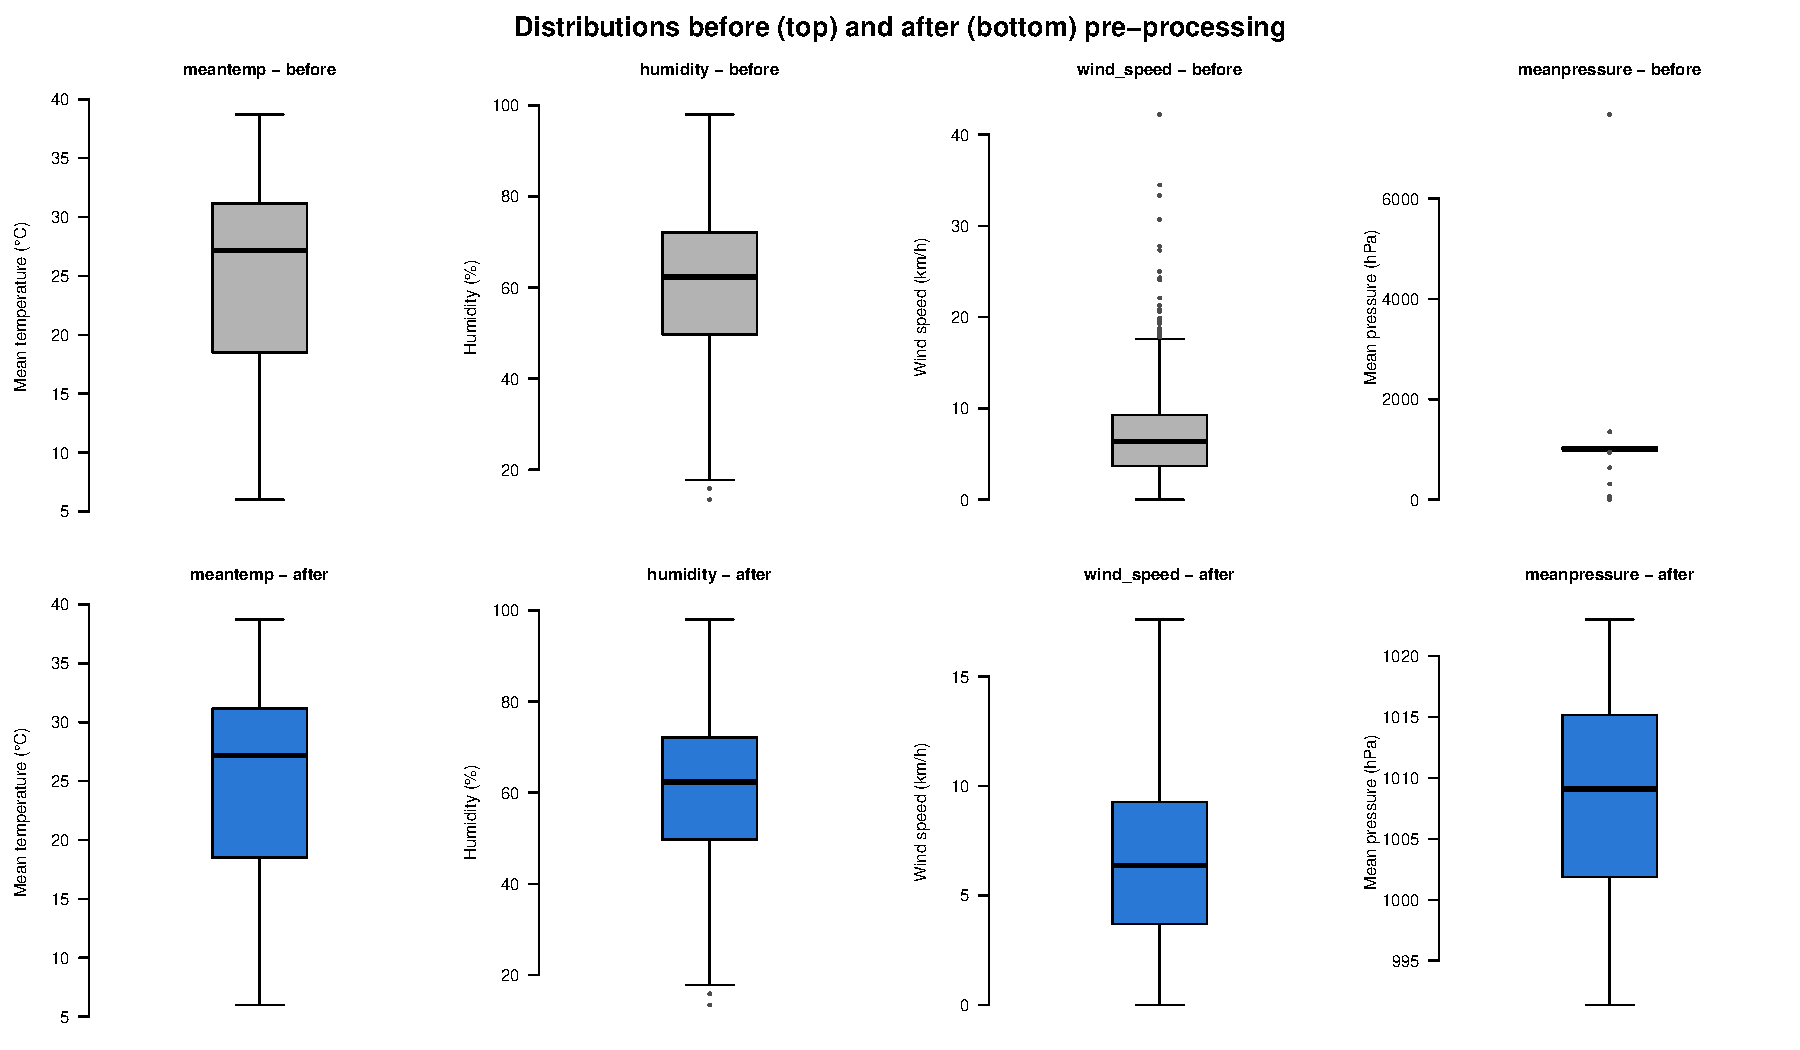
\includegraphics[width=\linewidth]{boxplots_before_after.pdf}
  \caption{Distributions before (top) and after (bottom) pre-processing. The raw pressure
           range is dominated by the invalid values; the wind speed outliers are capped.}
  \label{fig:box}
\end{figure}

\begin{figure}[htbp]
  \centering
  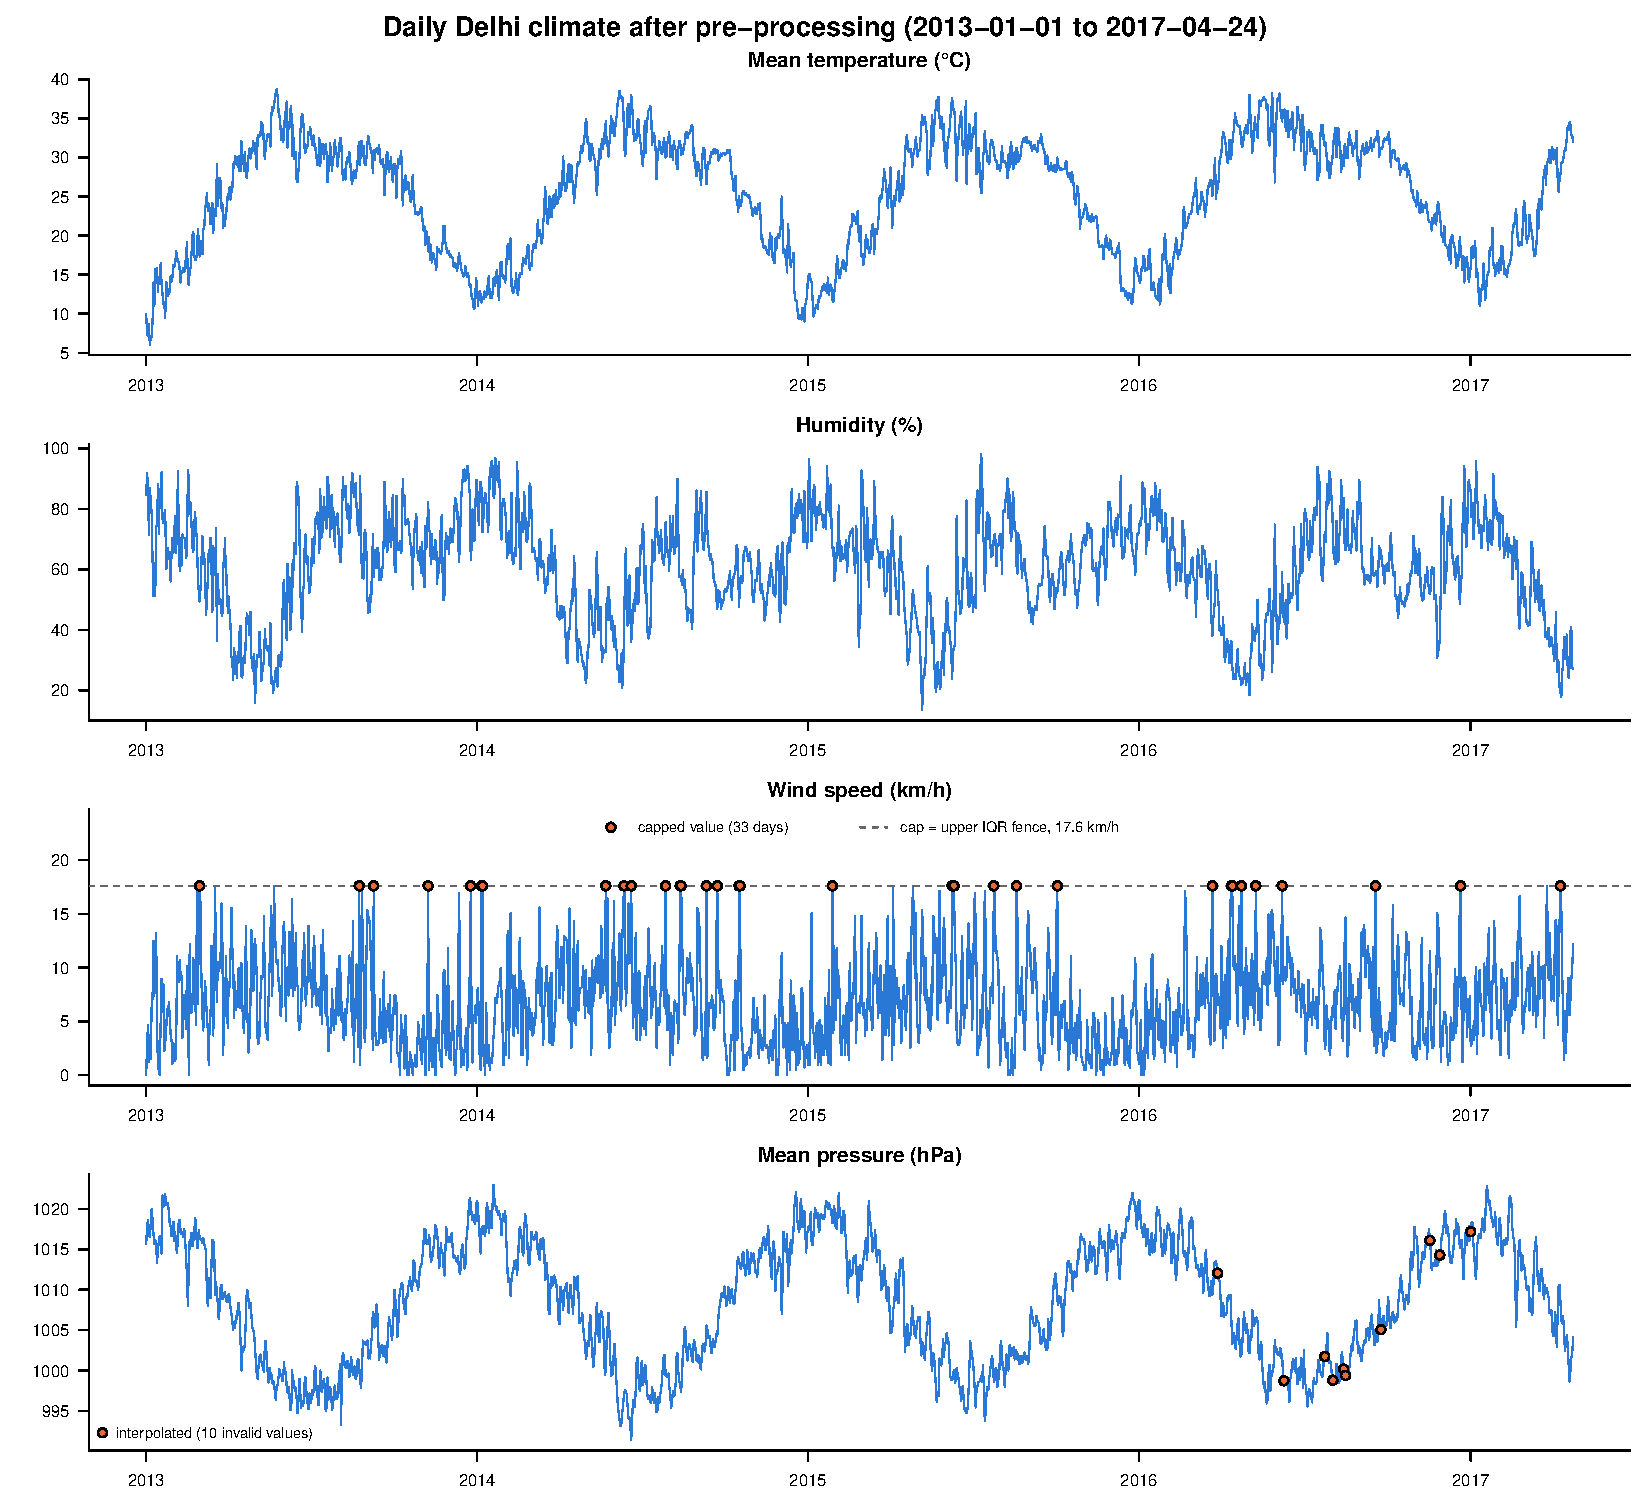
\includegraphics[width=\linewidth]{timeseries_clean.pdf}
  \caption{Cleaned daily series. Orange points mark the interpolated pressures (bottom panel) and the
           capped wind speeds (third panel). All four series show a clear annual cycle.}
  \label{fig:ts}
\end{figure}

% ---------------------------------------------------------------- 7
\section{Relation analysis between parameters (2b)}
\label{sec:corr}

Table~\ref{tab:correlation_pairs_ranked} ranks the six pairs by $|r|$ and
Figure~\ref{fig:heat} shows both correlation matrices.

\tabinput{correlation_pairs_ranked}

\begin{figure}[htbp]
  \centering
  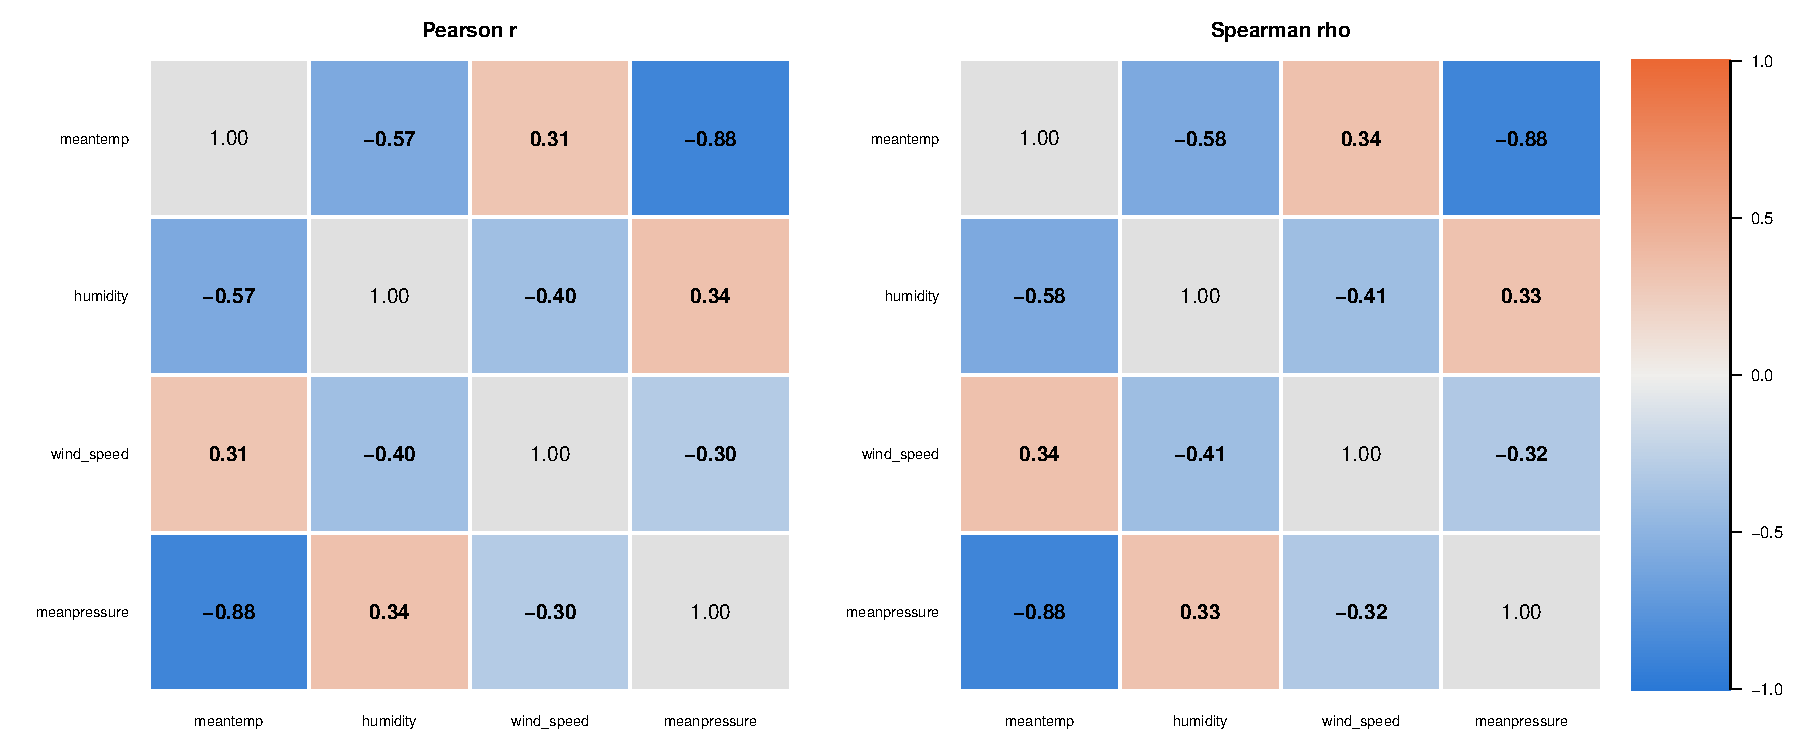
\includegraphics[width=\linewidth]{correlation_heatmaps.pdf}
  \caption{Pearson (left) and Spearman (right) correlation matrices.}
  \label{fig:heat}
\end{figure}

\paragraph{Key findings.}
\begin{itemize}
  \item \textbf{Temperature and pressure} are very strongly negatively correlated,
        $r=\rTP$ (95\% CI \rCIloTP{} to \rCIhiTP): hot days have low pressure.
  \item \textbf{Temperature and humidity}: strong negative, $r=\rTH$; hotter days are drier.
  \item \textbf{Humidity and wind speed} ($r=\rHW$), \textbf{humidity and pressure} ($r=\rHP$)
        and \textbf{temperature and wind speed} ($r=\rTW$) are moderate;
        \textbf{wind speed and pressure} is weak ($r=\rWP$).
  \item \textbf{Pearson and Spearman agree} for every pair (largest gap \maxRhoGap, for
        temperature--wind speed). There is therefore no sign of a curved
        \emph{monotonic} relation; both coefficients, however, are blind to
        non-monotonic patterns, which the scatter plots (Figure~\ref{fig:pairs}) do
        reveal: the temperature--humidity cloud splits into separate bands.
  \item All correlations are significant ($p<0.001$), \emph{even after} accounting for
        autocorrelation: the effective sample size drops to only \neffTP{} days for
        temperature--pressure (lag-1 autocorrelations \acfT{} and \acfP), but $|r|$ is
        so large that the relation remains clearly significant.
\end{itemize}

\begin{figure}[htbp]
  \centering
  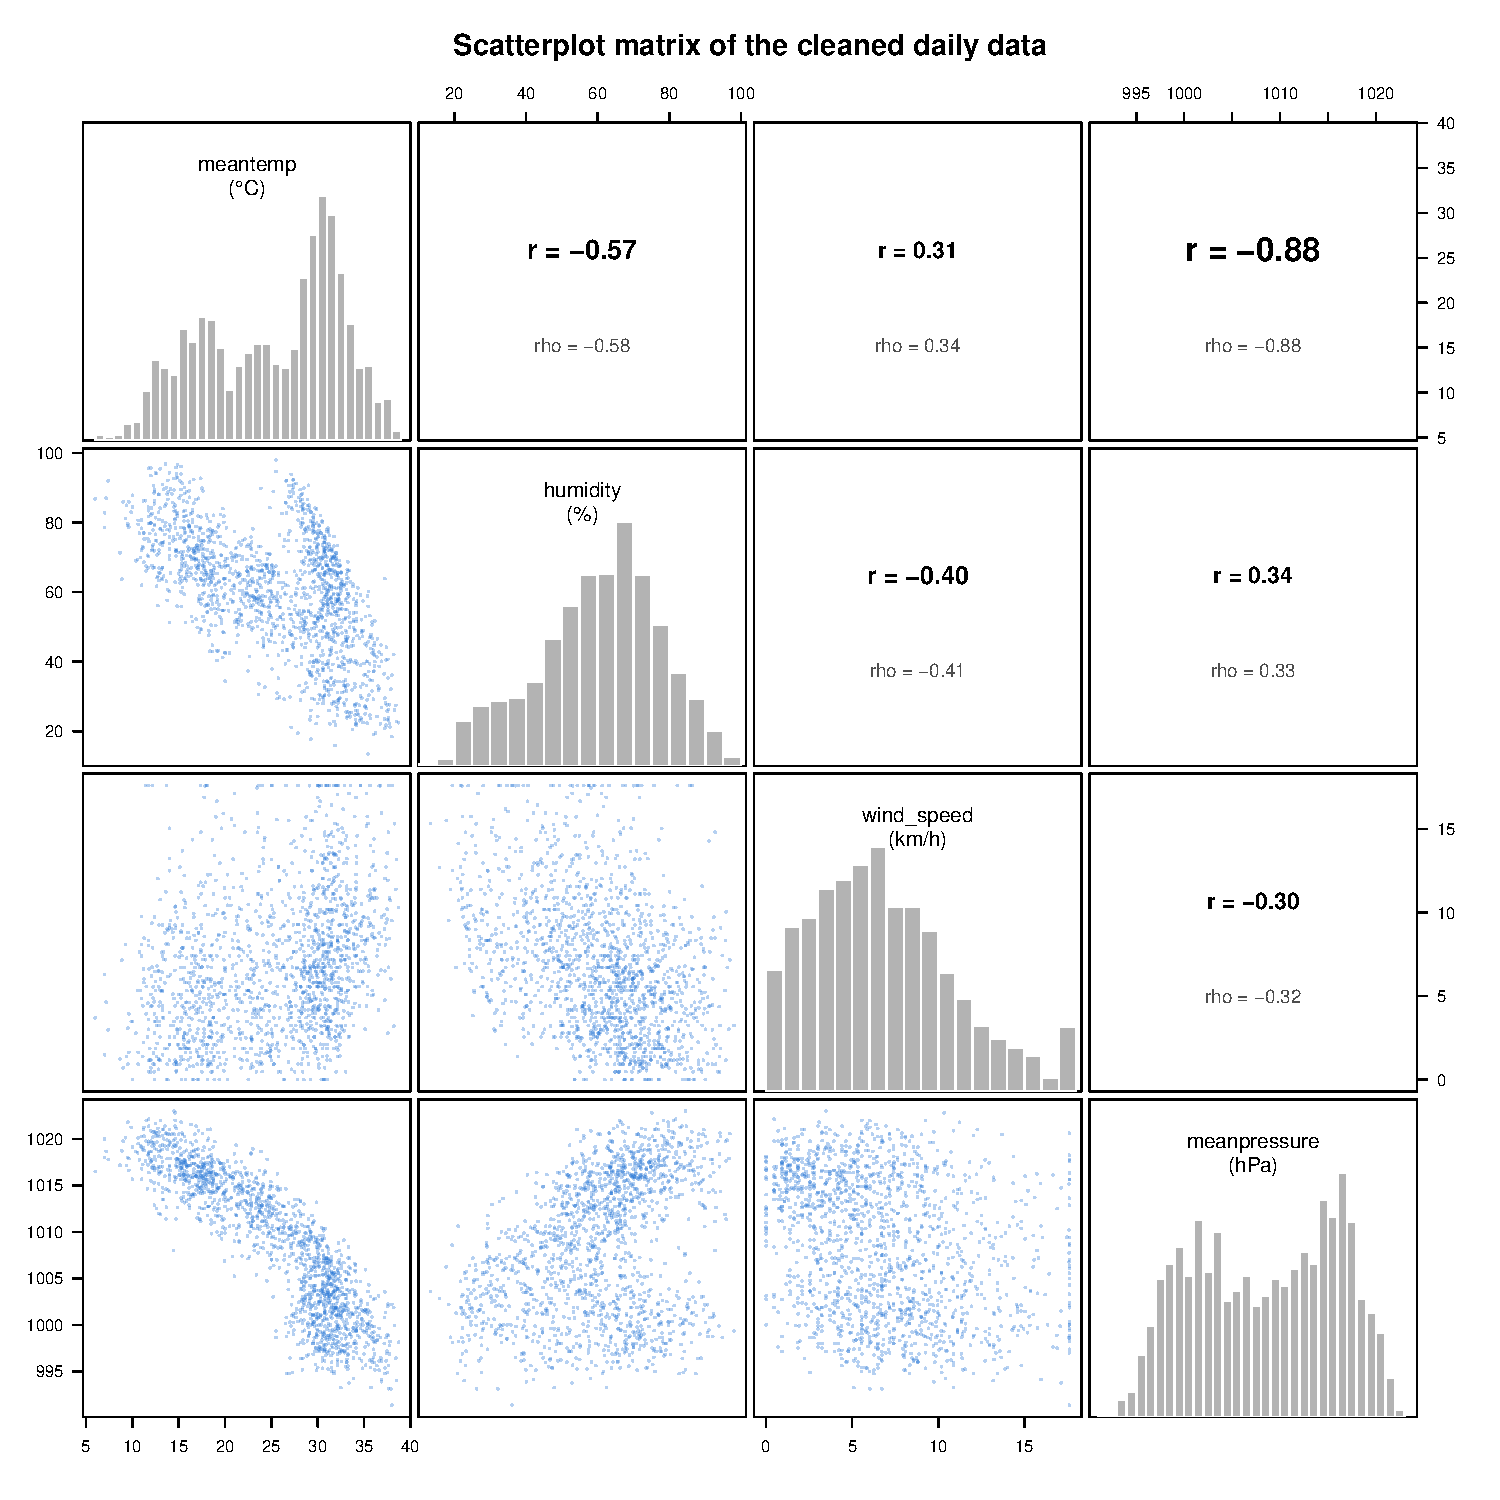
\includegraphics[width=0.85\linewidth]{scatterplot_matrix.pdf}
  \caption{Scatterplot matrix: scatter plots (lower), histograms (diagonal), Pearson $r$ and
           Spearman $\rho$ (upper).}
  \label{fig:pairs}
\end{figure}

\paragraph{Seasonal structure.} The calendar month alone explains \RmonthT\% of the daily
variance of temperature, \RmonthP\% of pressure, \RmonthH\% of humidity and only
\RmonthW\% of wind speed (Figure~\ref{fig:monthly}). Temperature peaks in May--June
and pressure is lowest in June--July; humidity has two maxima, in winter and in the monsoon
(July--August), and a deep minimum in the dry pre-monsoon months of April--May.
The year-by-year distributions (Figure~\ref{fig:year}) are similar for 2013--2016,
so the relations are not driven by one unusual year; 2017 differs only because it
covers January--April. This seasonal structure is the key to interpreting the
regressions below.

\begin{figure}[htbp]
  \centering
  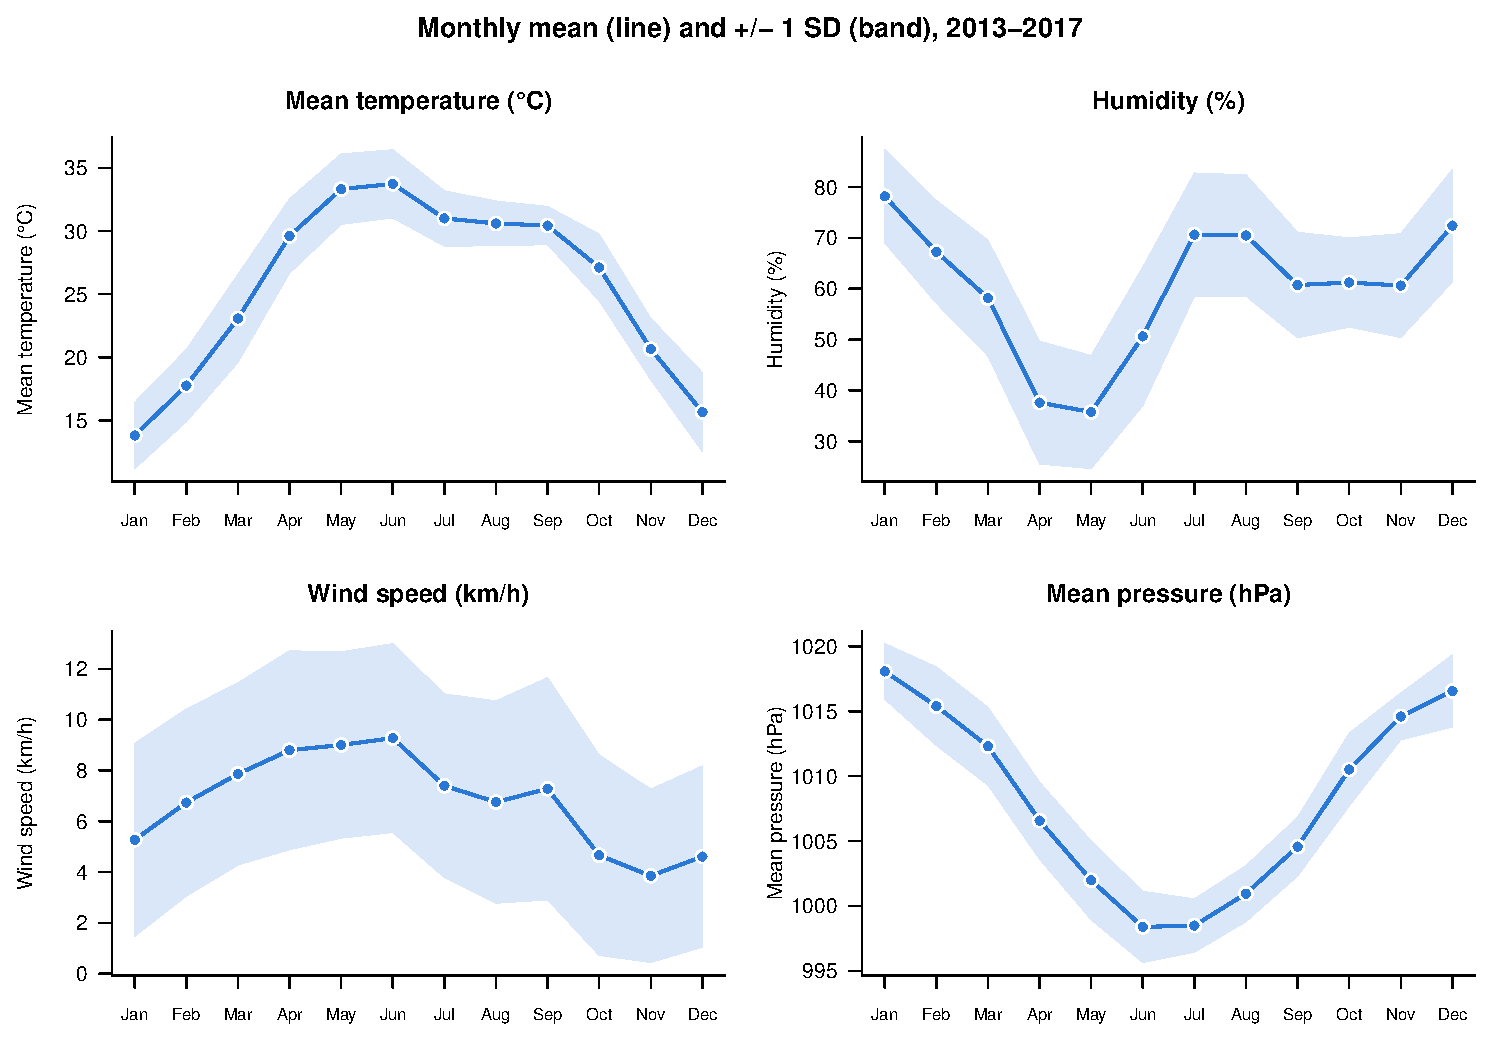
\includegraphics[width=0.95\linewidth]{monthly_profiles.pdf}
  \caption{Monthly mean and $\pm1$ standard deviation of each parameter (2013--2017).}
  \label{fig:monthly}
\end{figure}

\begin{figure}[htbp]
  \centering
  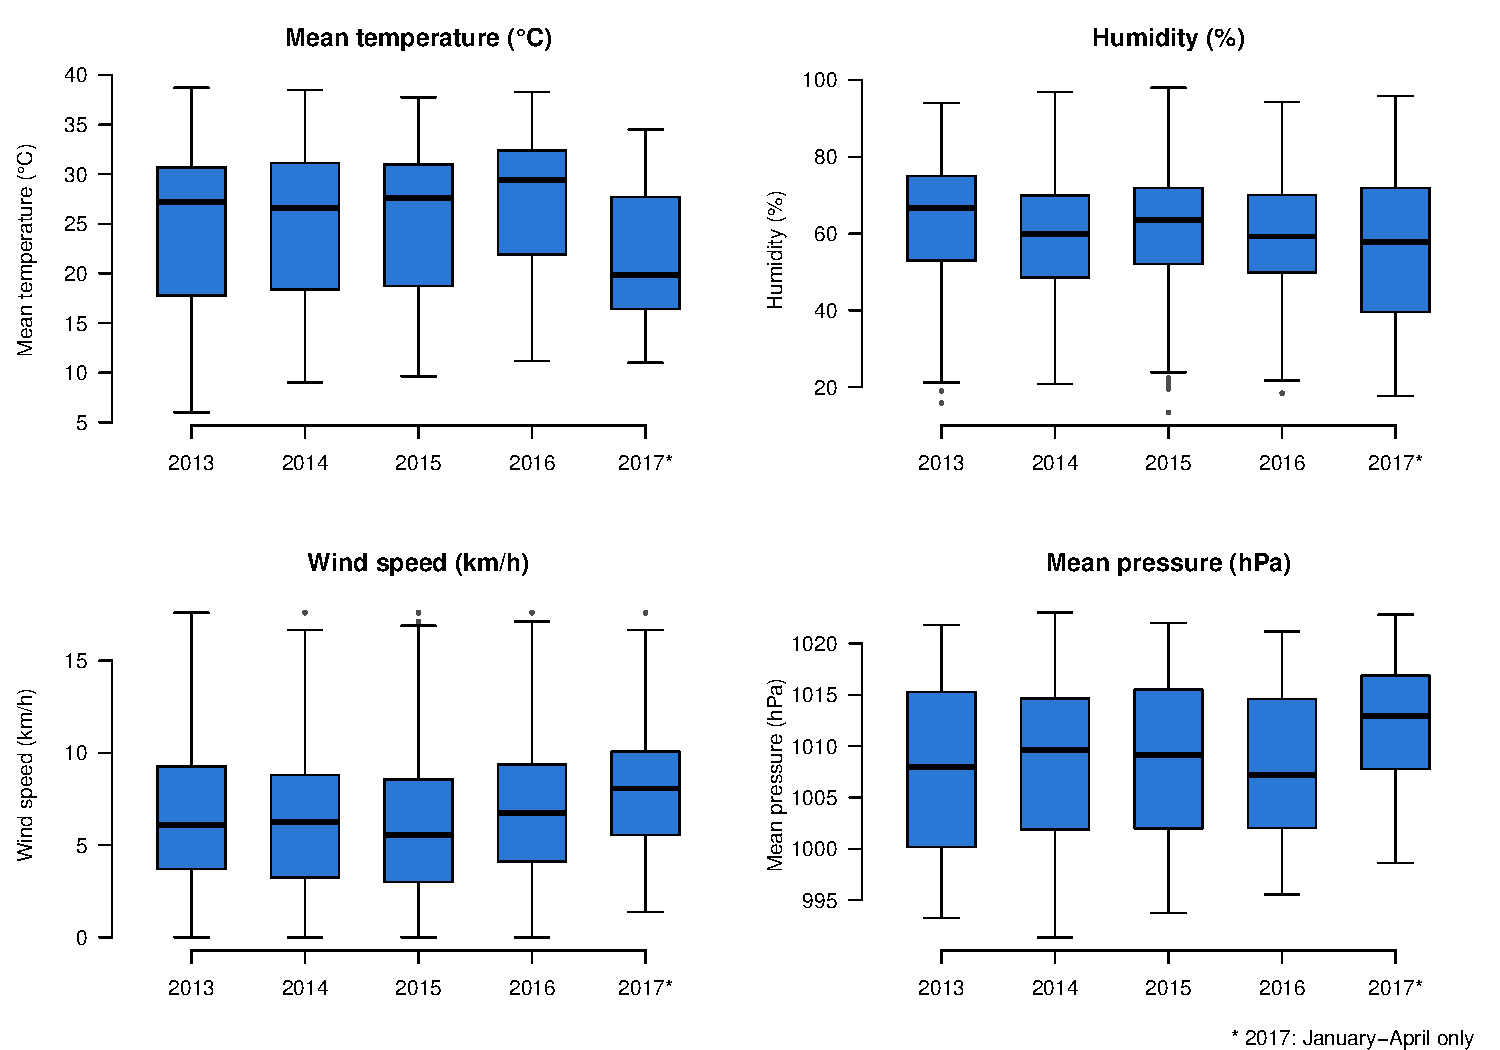
\includegraphics[width=0.95\linewidth]{boxplots_by_year.pdf}
  \caption{Distribution per year; 2017 covers January--April only, hence its lower
           temperatures and higher pressures.}
  \label{fig:year}
\end{figure}

% ---------------------------------------------------------------- 8
\section{Simple linear regression (2c-i)}
\label{sec:lin}

\paragraph{Direction of each model.} Mean temperature is the response for every pair
that contains it. For the other pairs we follow the chain from the large-scale state
to local weather: pressure drives wind, and both act on humidity, giving
\var{humidity}$\sim$\var{wind\_speed}, \var{humidity}$\sim$\var{meanpressure} and
\var{wind\_speed}$\sim$\var{meanpressure}. The direction is a modelling convention,
not a causal claim; the reverse fits are reported too. In simple regression $\Rsq=r^2$ in
both directions, but the slopes are not reciprocals: their product equals $r^2$
(e.g.\ $\slopeTP\times\slopeRevTP=\RlinTP$ for temperature and pressure).

\tabinput{linear_results}

\begin{figure}[htbp]
  \centering
  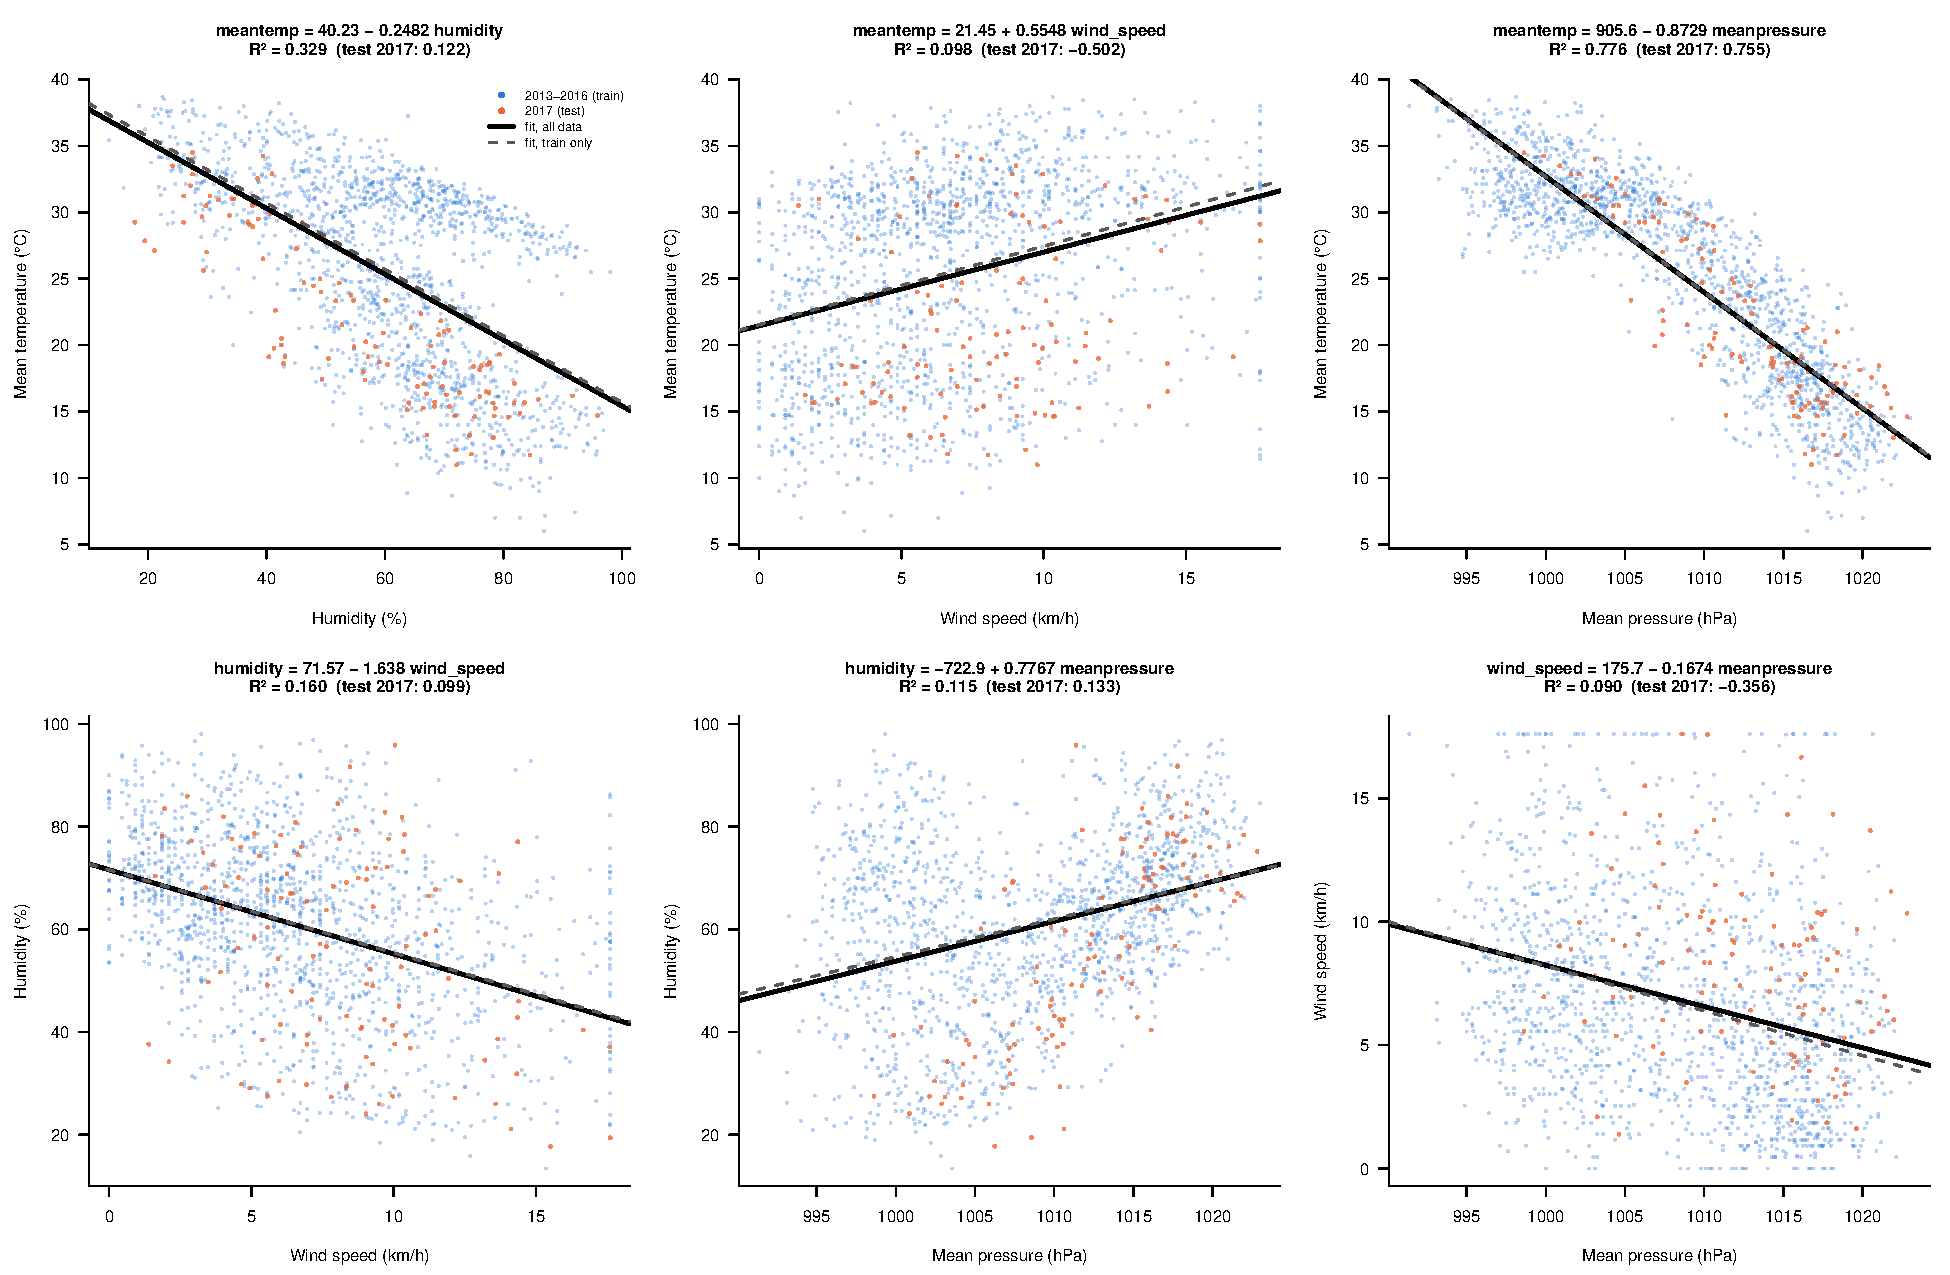
\includegraphics[width=\linewidth]{linear_fits.pdf}
  \caption{Linear fits on all data (solid) and on 2013--2016 only (dashed);
           blue: 2013--2016, orange: 2017 test days.}
  \label{fig:linfit}
\end{figure}

\paragraph{Results.} Table~\ref{tab:linear_results} lists all twelve linear fits and
Figure~\ref{fig:linfit} draws the six primary ones. The fitted temperature--pressure line is
$\widehat{\text{meantemp}}=\interceptTP\slopeTP\cdot\text{meanpressure}$: each additional
hPa of mean pressure goes with a change of \slopeTP\,$^\circ$C in mean temperature
(95\% CI \slopeCIloTP{} to \slopeCIhiTP), and pressure alone explains \RlinTP{} of the
variance of temperature. The line generalises well: fitted on 2013--2016 it reaches
$\Rsq_{\text{test}}=\RlinTestTP$ on 2017. Humidity explains \RlinTH{} of the temperature
variance (slope \slopeTH\,$^\circ$C per \% humidity), but only \RlinTestTH{} on the 2017 test
period. The other four linear relations have $\Rsq$ between \RlinWP{} and \RlinHW;
for temperature--wind speed and wind speed--pressure the test $\Rsq$ is even negative
(\RlinTestTW{} and \RlinTestWP), i.e.\ the lines predict the January--April 2017 days
worse than their mean. The test period covers a single season with a narrower range
of values, so a low test $\Rsq$ partly reflects that narrower range and not only a
poor fit.

\paragraph{Residual diagnostics.} Figure~\ref{fig:linres} shows the residuals against
the fitted values with binned means as a simple smoother. For temperature--pressure
the binned means trace an inverted U: the line underestimates temperatures in the
middle of the range and overestimates them at both ends, a sign of curvature.
Humidity--pressure shows the opposite U-shape. For temperature--humidity the residuals
split into two bands (monsoon days above, winter days below) rather than a curve. The
Q--Q plots (Figure~\ref{fig:qq}) show light tails for temperature--humidity (a mixture
of regimes) and right skew for wind speed--pressure. The Durbin--Watson statistics lie
between \DWmin{} and \DWmax{}, far below~2: the residuals are strongly
autocorrelated, so the standard errors and $p$-values above are optimistic. The
slopes and $\Rsq$ values remain valid as descriptions of the fitted relation.

\begin{figure}[htbp]
  \centering
  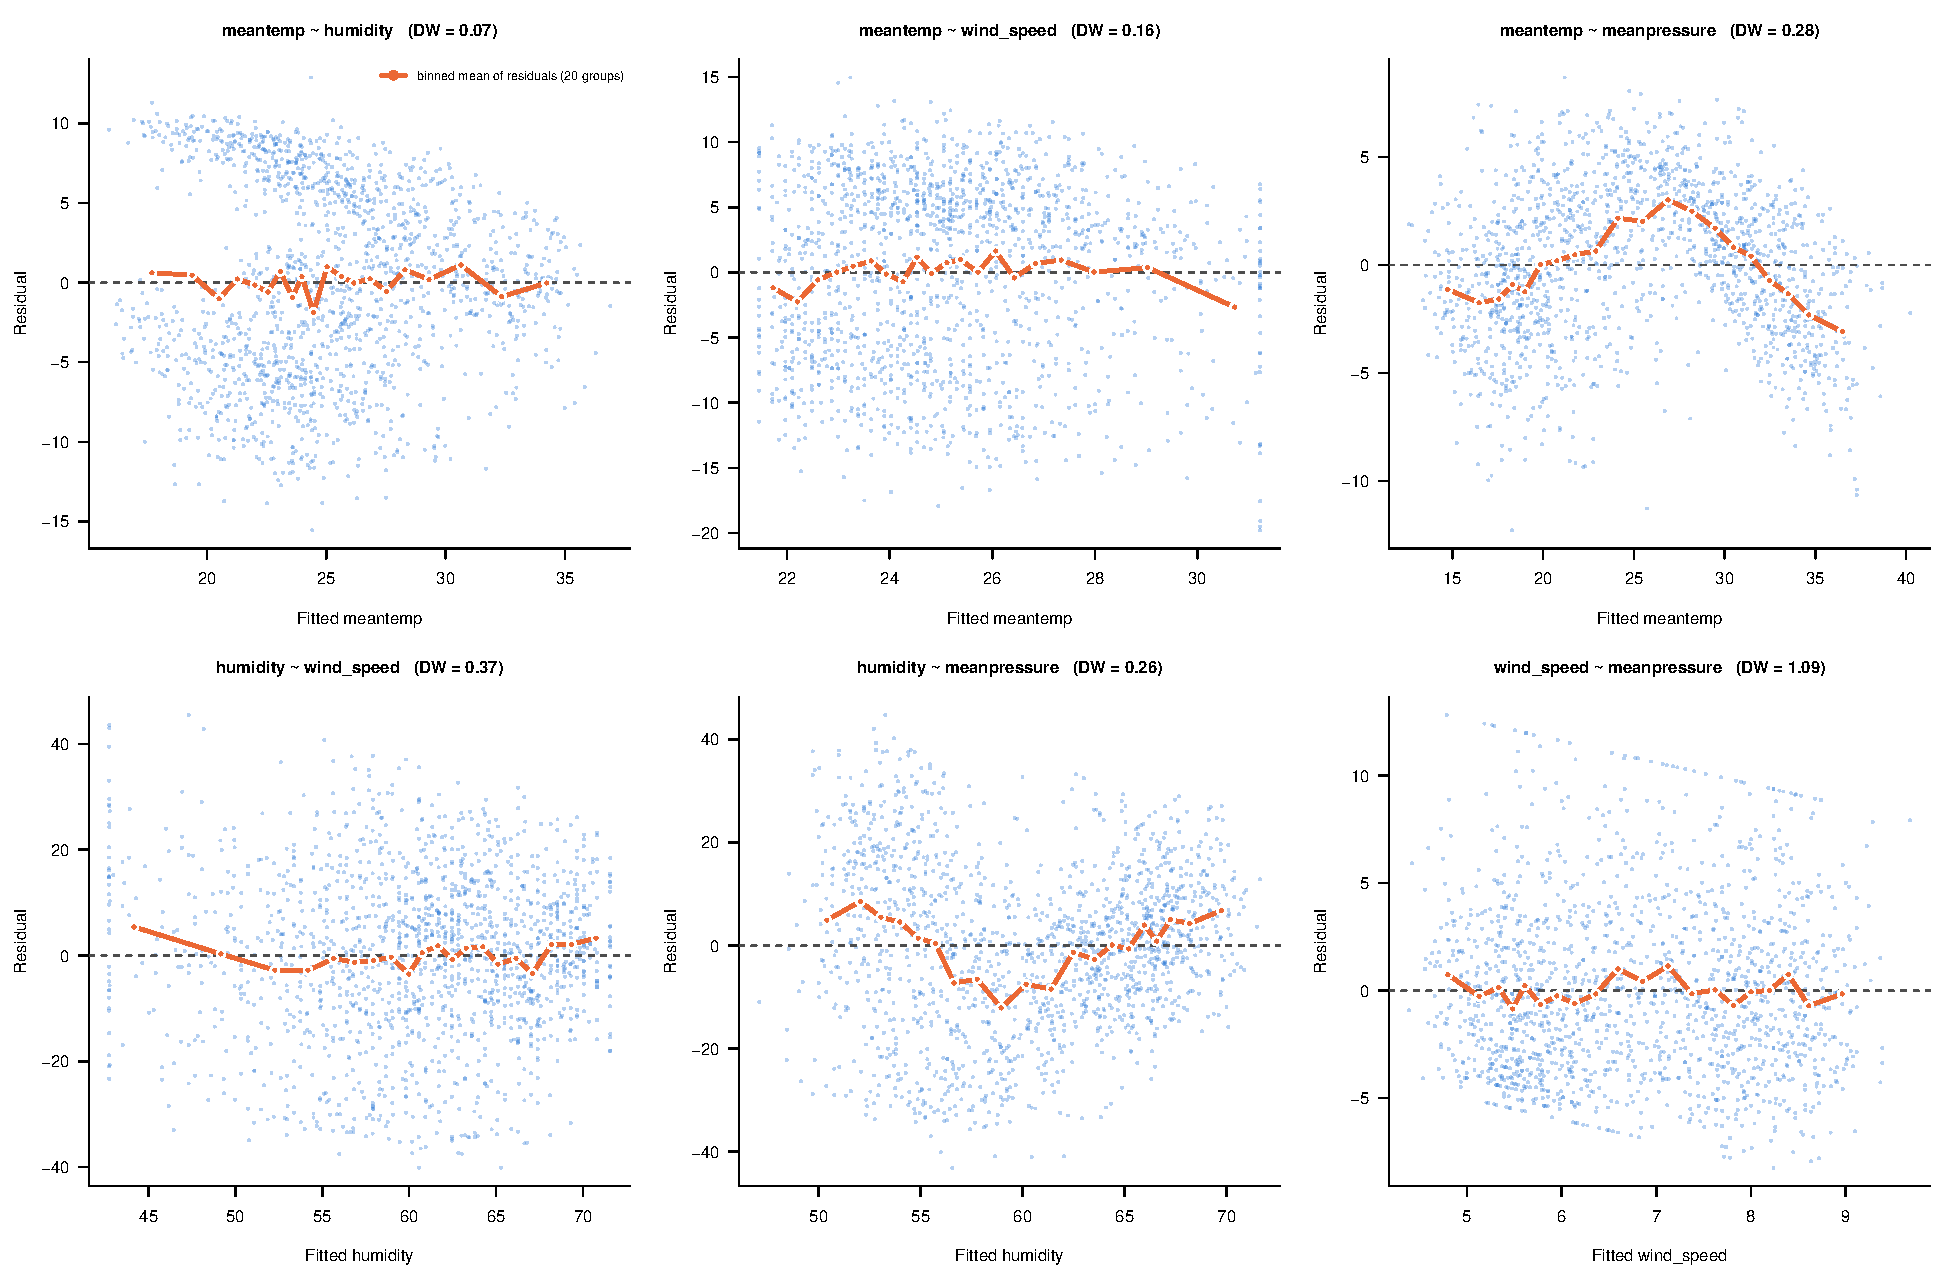
\includegraphics[width=\linewidth]{linear_residuals_vs_fitted.pdf}
  \caption{Residuals vs fitted values of the linear models; orange: mean residual in 20
           equal-size groups.}
  \label{fig:linres}
\end{figure}

\begin{figure}[htbp]
  \centering
  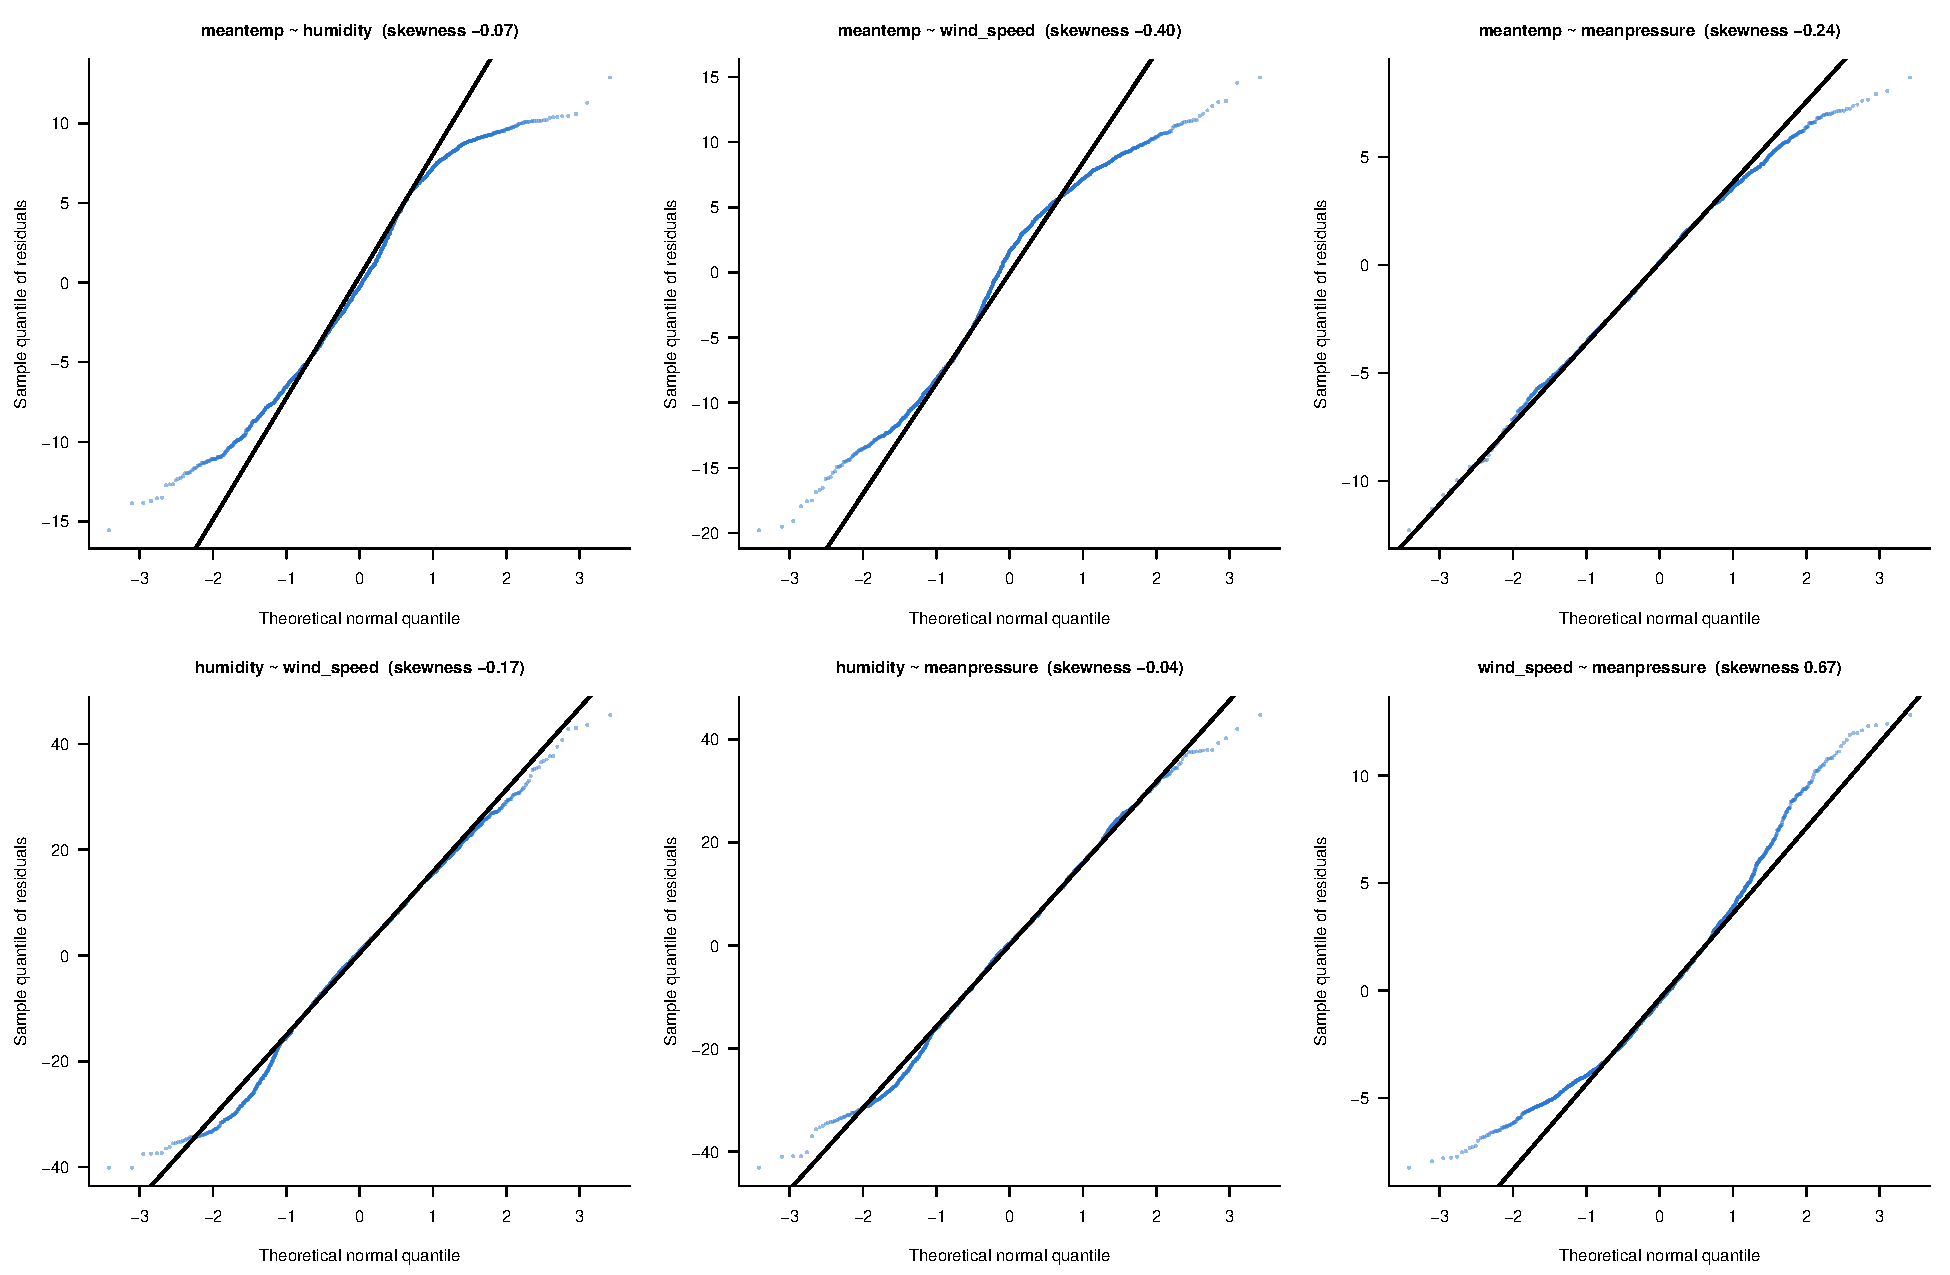
\includegraphics[width=\linewidth]{linear_qq.pdf}
  \caption{Normal Q--Q plots of the linear residuals.}
  \label{fig:qq}
\end{figure}

% ---------------------------------------------------------------- 9
\section{Simple non-linear regression (2c-ii)}
\label{sec:nl}

The five curves of Section~\ref{sec:method-nl} were fitted to the same six pairs
and directions (60 non-linear fits, plus the linear reference). All \nGNtotal{}
exponential and power fits converged, in \GNitMin--\GNitMax{} Gauss--Newton
iterations; \nSkipped{} fits (logarithmic and power with wind speed as predictor)
were skipped because $\ln x$ is undefined at zero wind speed. Table~\ref{tab:nonlinear_results}
lists every curve for the primary directions (the reverse directions are in the
CSV file), Table~\ref{tab:nonlinear_best} compares the selected curve with the line
for all twelve relations, and Figure~\ref{fig:nlfit} draws all curves.

\tabinput{nonlinear_results}

\begin{figure}[htbp]
  \centering
  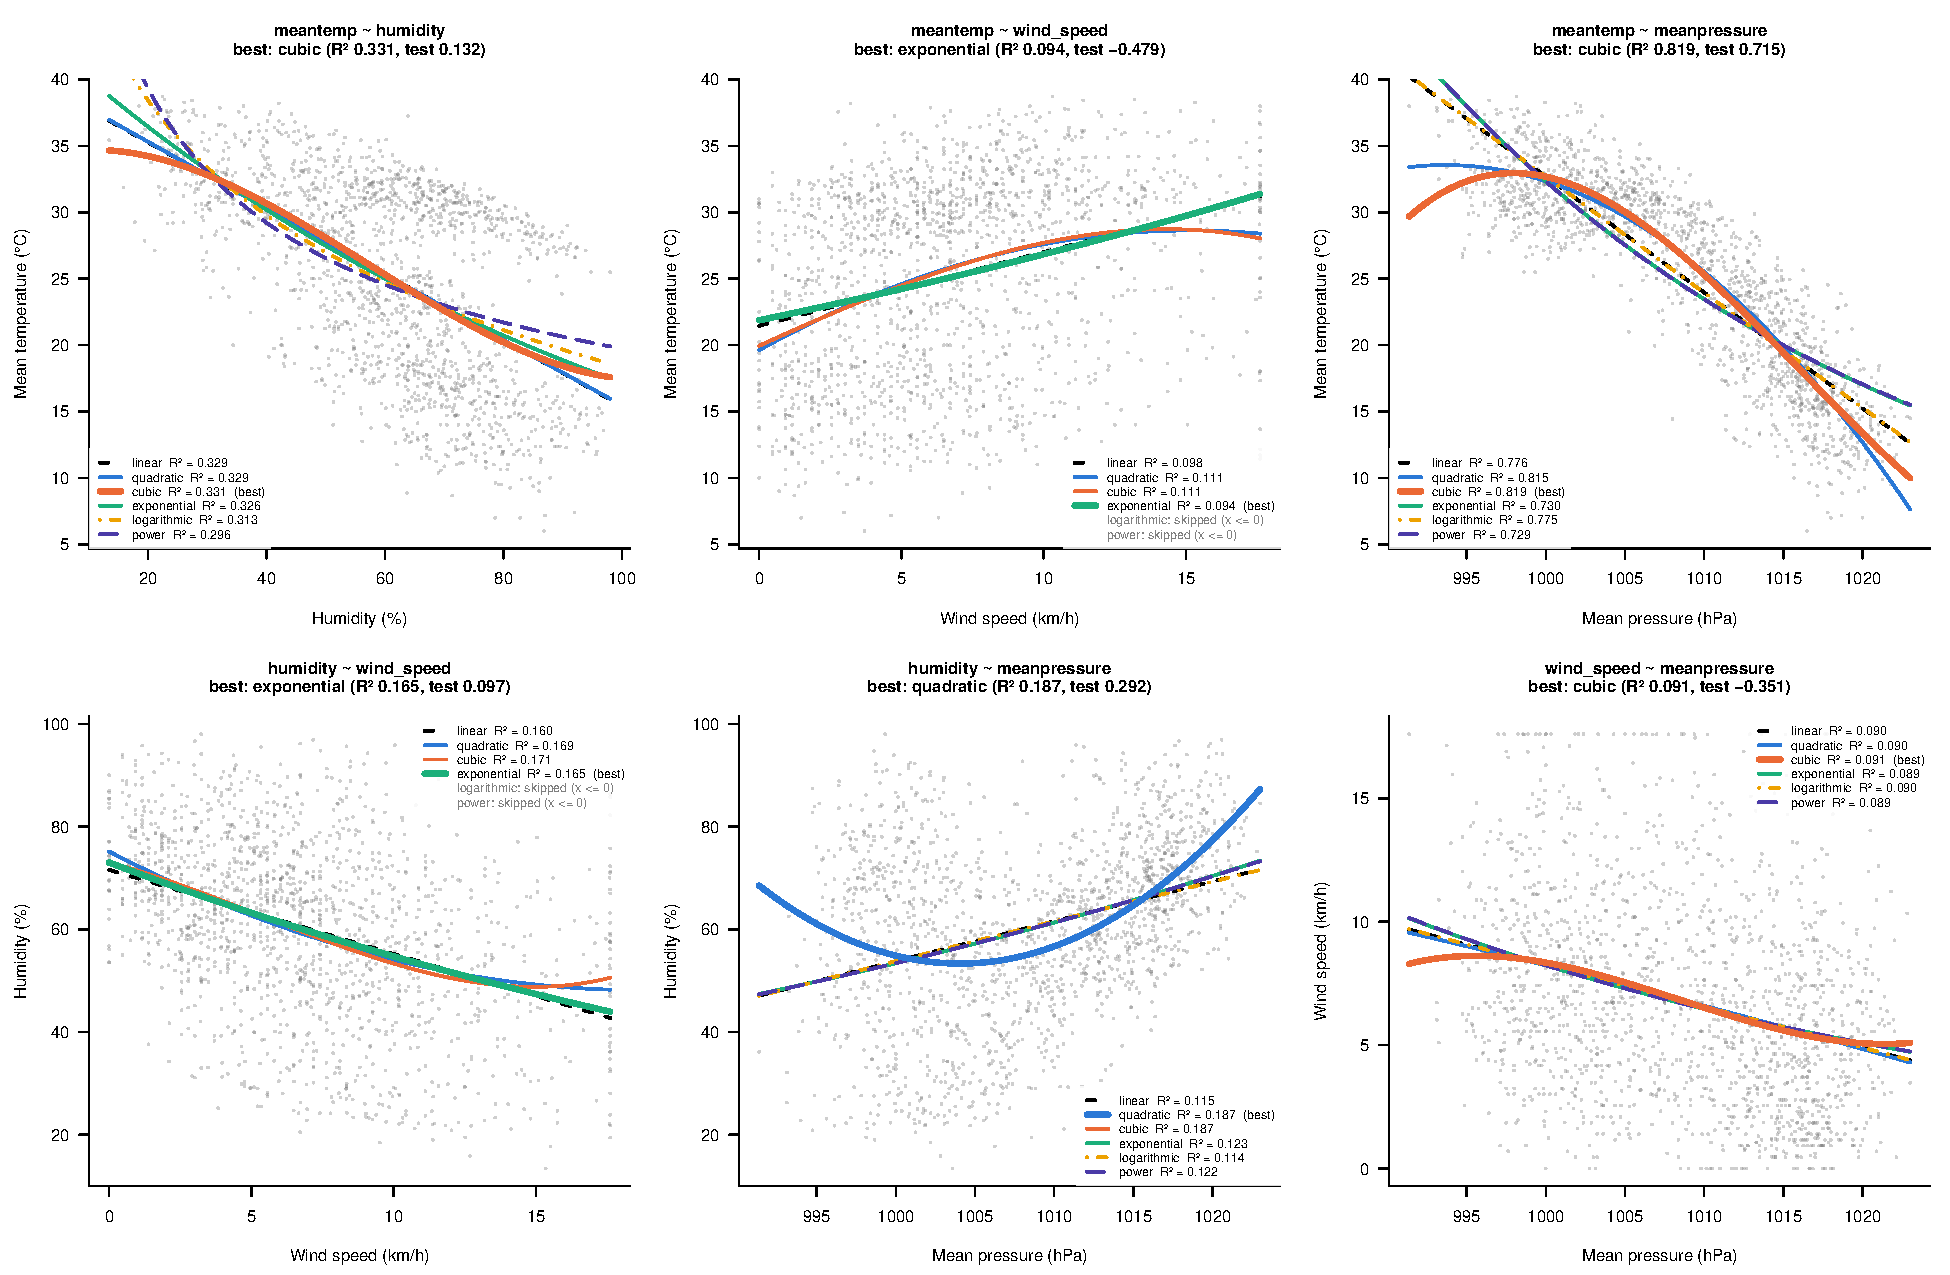
\includegraphics[width=\linewidth]{nonlinear_fits.pdf}
  \caption{All fitted curves per pair; the selected curve is drawn thick.}
  \label{fig:nlfit}
\end{figure}

\tabinput{nonlinear_best}

\paragraph{Results per relation.}
\begin{itemize}
  \item \textbf{Humidity--pressure}: the quadratic raises $\Rsq$ from \RlinHP{} to
        \RbestHP{} ($\Delta\Rsq=\gainHP$), and the gain is confirmed out of sample
        (test $\Rsq$ \RlinTestHP{} $\rightarrow$ \RbestTestHP). The U-shape is real in the
        data but reflects the order of the seasons along the pressure axis: humid
        low-pressure monsoon days, dry pre-monsoon days at intermediate pressure and
        humid high-pressure winter days.
  \item \textbf{Temperature--pressure}: the cubic removes the curvature seen in the linear
        residuals and raises $\Rsq$ from \RlinTP{} to \RbestTP{} ($\Delta\Rsq=\gainTP$).
        The test $\Rsq$, however, falls from \RlinTestTP{} to \RbestTestTP, because the
        curvature lies at summer temperatures that the January--April test period does
        not contain. The cubic also peaks at \cubicPeakTP\,hPa and turns down at the lowest
        pressures, where few days lie, so it must not be extrapolated.
  \item \textbf{Temperature--humidity}: the best curve (\bestTH) adds only \gainTH{} to
        $\Rsq$. No function of humidity alone can separate the monsoon band from the rest.
  \item \textbf{Relations with wind speed}: the curves change $\Rsq$ by at most
        \maxGainTW{} (temperature), \maxGainHW{} (humidity) and \maxGainWP{} (pressure);
        a straight line is adequate. For temperature--wind speed the selected exponential
        even has a slightly \emph{lower} $\Rsq$ than the line (\gainTW) and was chosen only
        for a marginally better test $\Rsq$.
\end{itemize}

\paragraph{Overfitting.} For \nOverfit{} of the 12 relations the cubic beats the
quadratic on adjusted $\Rsq$ but loses on the test period; the selection score
(Section~\ref{sec:selection}) therefore rejects several in-sample gains, e.g.\ the
cubic for temperature--wind speed (\maxGainTW). The residuals of the selected curves
(Figure~\ref{fig:nlres}) no longer show systematic curvature, but their Durbin--Watson
statistics remain far below~2.

\begin{figure}[htbp]
  \centering
  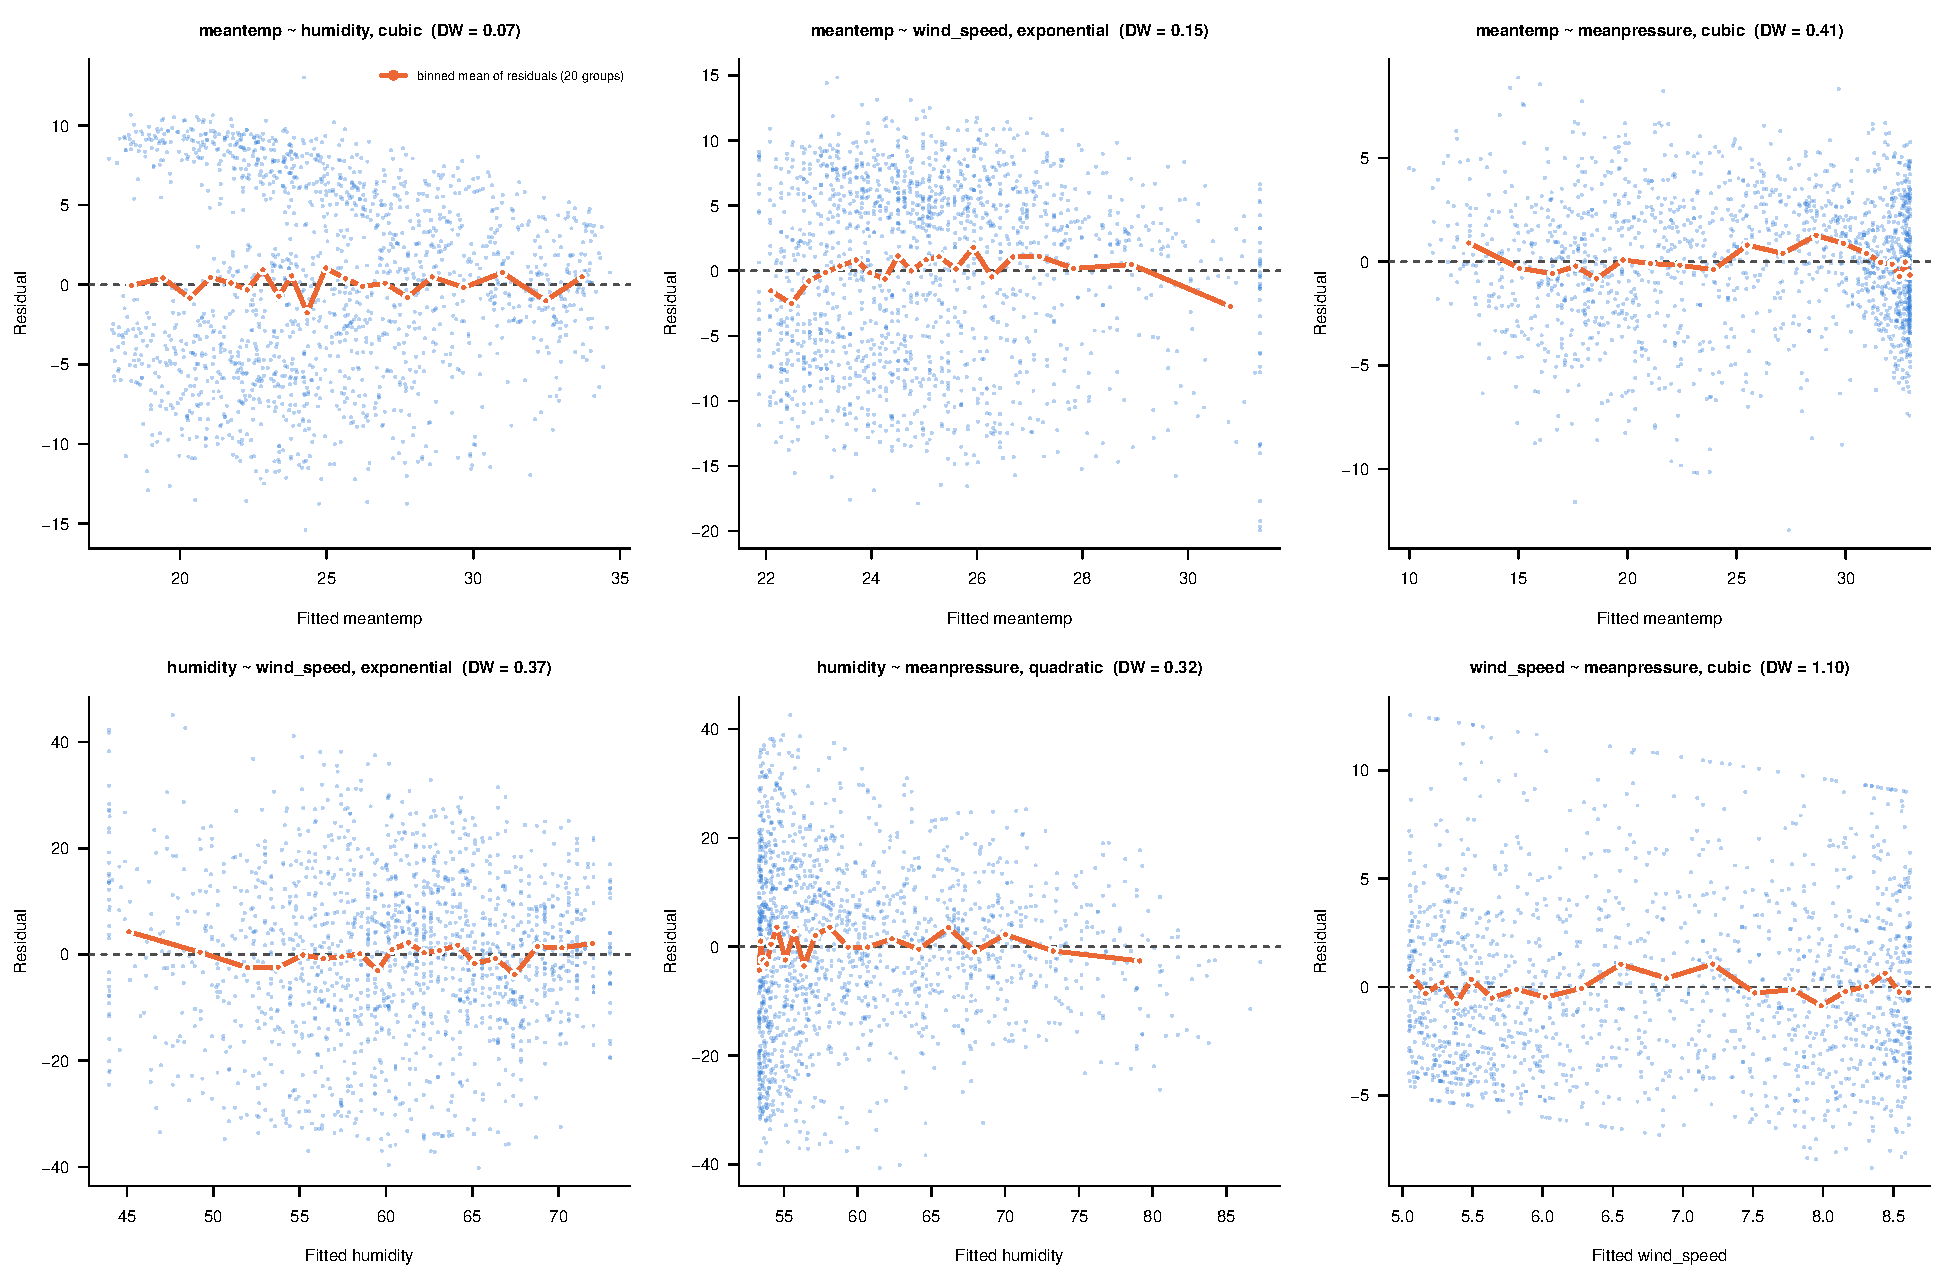
\includegraphics[width=\linewidth]{nonlinear_best_residuals.pdf}
  \caption{Residuals of the selected curve for each pair, with binned means.}
  \label{fig:nlres}
\end{figure}

% ---------------------------------------------------------------- 10
\section{\texorpdfstring{$R^2$}{R2} comparison and discussion (2d)}
\label{sec:r2}

Table~\ref{tab:r2_comparison} collects the $\Rsq$ of every curve for every relation,
Figure~\ref{fig:r2heat} shows the linear and selected $\Rsq$ as matrices and
Figure~\ref{fig:gain} the gain of the best non-linear curve over the line.

\tabinput{r2_comparison}

\begin{figure}[htbp]
  \centering
  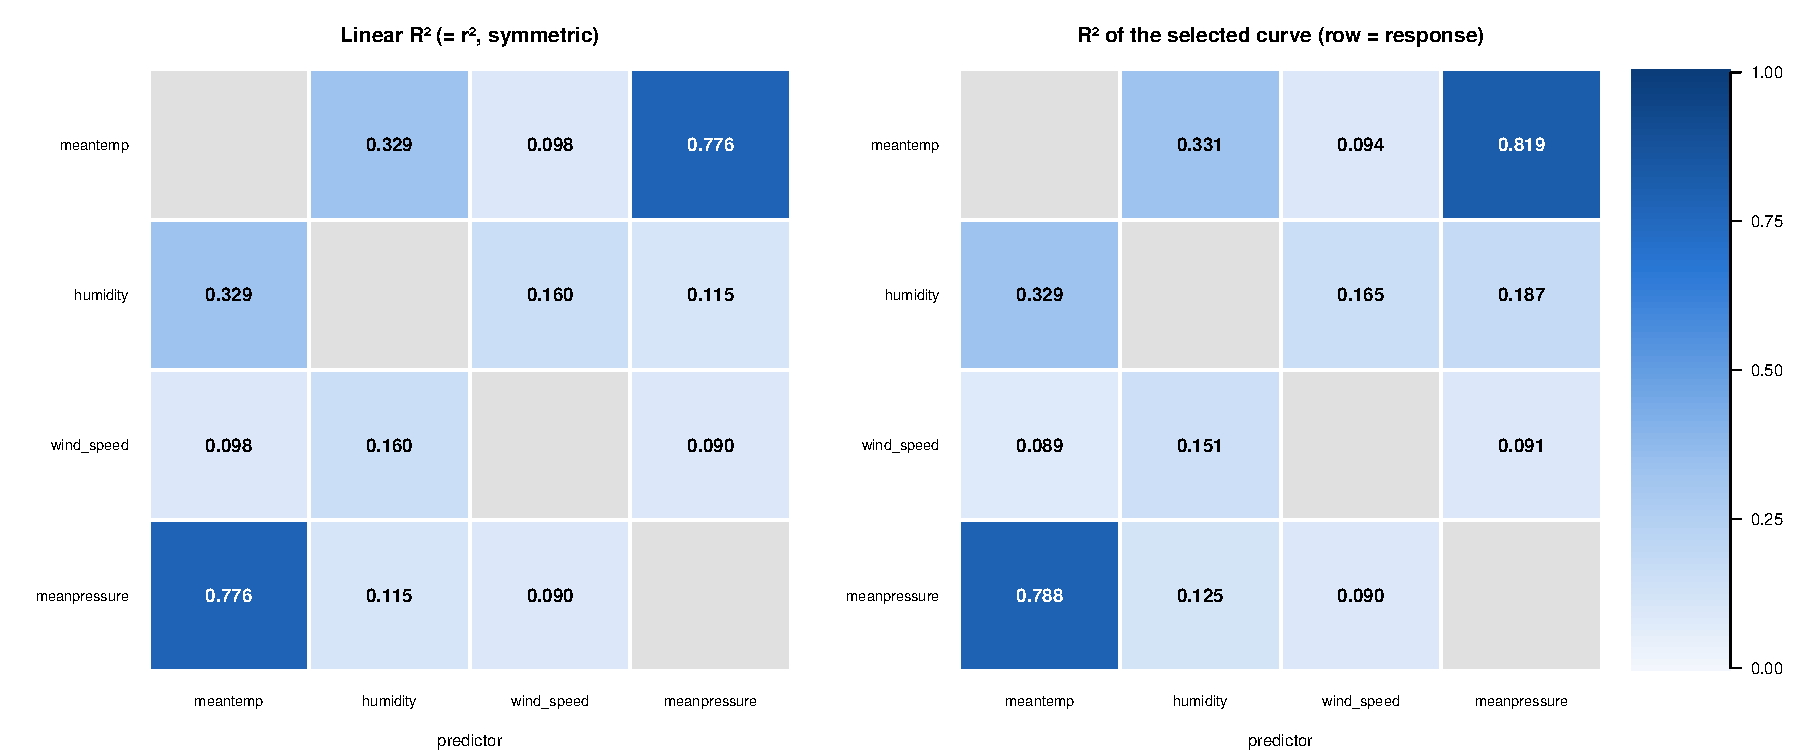
\includegraphics[width=\linewidth]{r2_heatmaps.pdf}
  \caption{Linear $\Rsq$ ($=r^2$, symmetric) and $\Rsq$ of the selected curve (row = response).}
  \label{fig:r2heat}
\end{figure}

\begin{figure}[htbp]
  \centering
  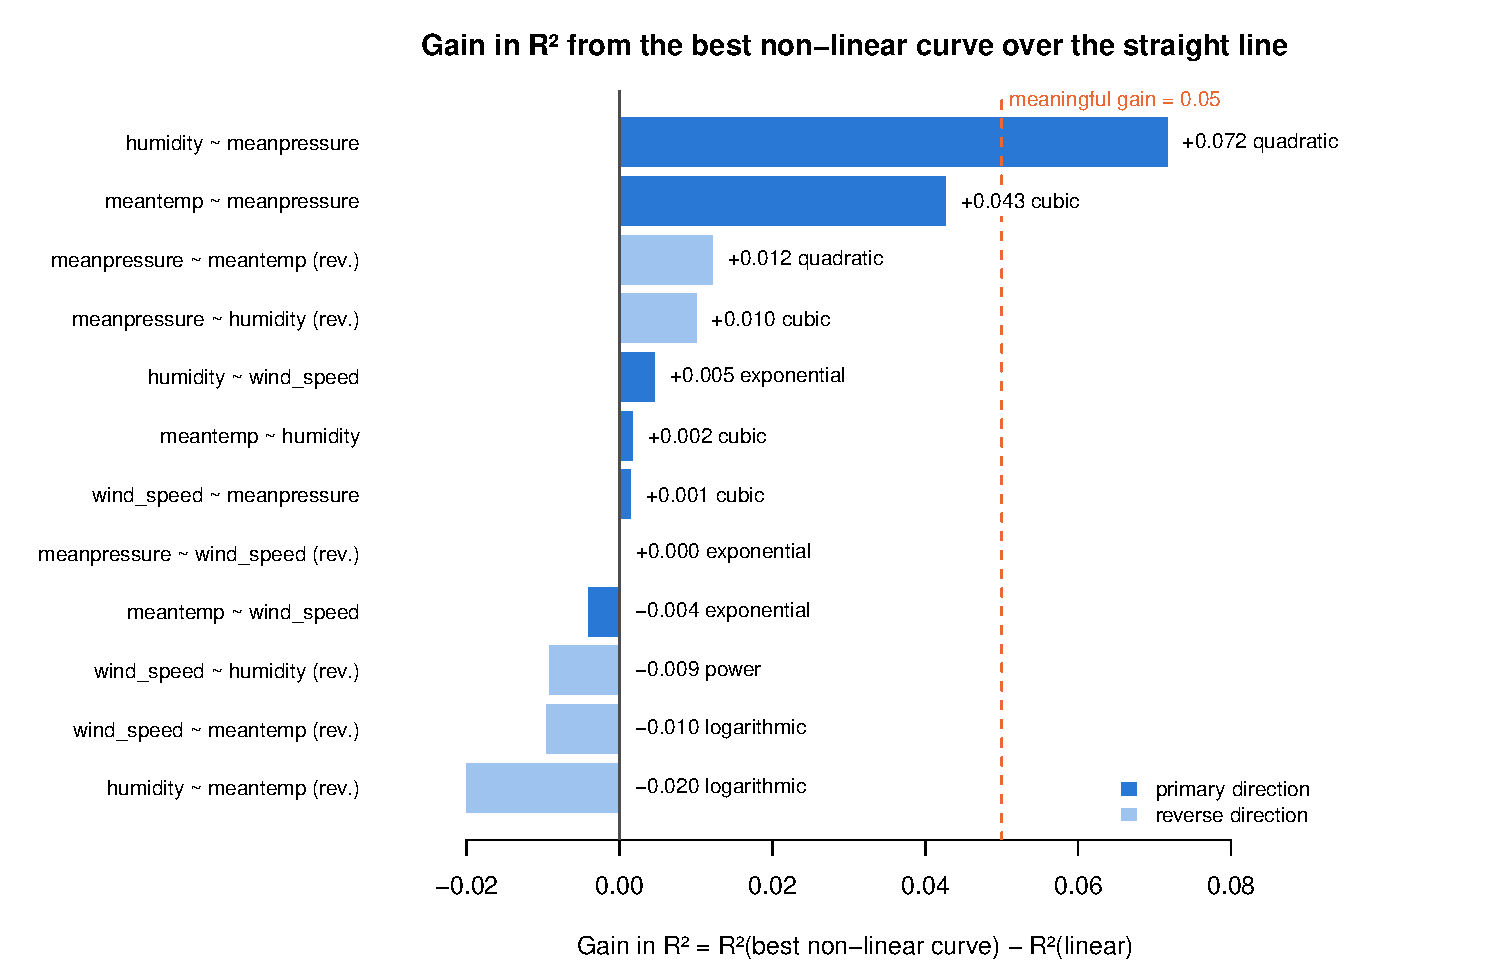
\includegraphics[width=0.85\linewidth]{r2_gain_barplot.pdf}
  \caption{Gain in $\Rsq$ of the best non-linear curve over the straight line; dashed:
           threshold for a meaningful gain (0.05).}
  \label{fig:gain}
\end{figure}

Table~\ref{tab:relations_ranked} ranks the six relations by the $\Rsq$ of their selected
curve and adds, in the last column, the $\Rsq$ that remains once the annual cycle is
removed; the two rankings differ markedly, which the seasonality discussion below explains.

\tabinput{relations_ranked}

\paragraph{Are the high $\Rsq$ values driven by a few outliers?} No. Removing the
\nInflMin--\nInflMax{} days with Cook's $D>4/n$ changes the linear $\Rsq$ by
\cookMin{} to \cookMax{} (Table~\ref{tab:robustness_check}): it \emph{rises} in every
case, so the influential days are poorly fitted days that lower the fit, and no
reported $\Rsq$ is inflated by a few extreme observations. The wind-speed capping
does matter slightly: with the raw wind speeds the linear $\Rsq$ would be
\RrawWindTW, \RrawWindHW{} and \RrawWindWP{} instead of \RlinTW, \RlinHW{} and \RlinWP.
Part of these (weak) relations therefore depends on that pre-processing decision,
although the conclusion ``weak'' does not change.

\tabinput{robustness_check}

\paragraph{Seasonality.} Table~\ref{tab:seasonality_check} compares the correlation of
the raw data with the correlation of the anomalies (annual cycle removed) and within
each season.
\begin{itemize}
  \item \textbf{Temperature--pressure} is largely seasonal: $r$ falls from \rTP{} to \ranomTP{}
        on the anomalies, so \seasShareTP\% of the $\Rsq$ is the shared annual cycle (hot,
        low-pressure summer and monsoon vs.\ cool, high-pressure winter). A real
        day-to-day link remains, strongest within the pre-monsoon season ($r=\rSummerTP$)
        and weakest in the monsoon ($r=\rMonsoonTP$).
  \item \textbf{Temperature--humidity} is \emph{not} mainly seasonal: $r$ changes only from
        \rTH{} to \ranomTH{} (\seasShareTH\% seasonal), and within the summer and the
        monsoon the relation is even stronger ($r=\rSummerTH$ and \rMonsoonTH). Mixing the
        seasons \emph{weakens} the overall correlation, because monsoon days are both hot
        and humid (on average \monsoonTemp\,$^\circ$C and \monsoonHum\% humidity) and form
        a separate band. This is why the overall $\Rsq$ is only moderate and why no single
        curve in humidity improves it.
  \item \textbf{Humidity--pressure} (\seasShareHP\% seasonal), \textbf{temperature--wind speed}
        (\seasShareTW\%) and \textbf{wind speed--pressure} (\seasShareWP\%) are mostly
        seasonal; the humidity--pressure relation is strong within the pre-monsoon season
        ($r=\rSummerHP$) but absent in the monsoon ($r=\rMonsoonHP$).
\end{itemize}

\tabinput{seasonality_check}

\paragraph{What the regressions do not show.} Our temperature--pressure model predicts
temperature \emph{from} pressure, but that is only the direction we chose for the
regression. Physically the chain runs, if anything, the other way: strong heating of
north India in \hotMonth{} goes together with the seasonal low pressure over the region,
while the cool winter air mass brings high pressure. Both variables follow the
same annual forcing, which is exactly why removing the monthly means
(Table~\ref{tab:seasonality_check}) removes most of their correlation. The same caution
applies to every pair: a high $\Rsq$ here means that one parameter is a good
\emph{statistical} predictor of another in Delhi's climate, not that changing one
would change the other.

% ---------------------------------------------------------------- 11
\section{Conclusion}
\label{sec:conclusion}

\begin{enumerate}
  \item \textbf{Strongest relation: temperature and pressure.} $r=\rTP$; a straight line
        explains \RlinTP{} of the temperature variance (slope \slopeTP\,$^\circ$C/hPa) and
        the cubic \RbestTP. The line generalises to 2017 ($\Rsq_{\text{test}}=\RlinTestTP$),
        the cubic less well (\RbestTestTP). About \seasShareTP\% of this $\Rsq$ is the
        shared annual cycle.
  \item \textbf{Moderate relation: temperature and humidity.} $r=\rTH$, linear $\Rsq=\RlinTH$;
        non-linear curves add nothing ($\Delta\Rsq=\gainTH$). This relation survives the
        removal of the seasons (anomaly $r=\ranomTH$) and is a genuine day-to-day link:
        hotter days are drier in every season (only weakly so in the post-monsoon season, $r=\rPostTH$).
  \item \textbf{Weak relations:} humidity--wind speed ($\Rsq=\RlinHW$) and humidity--pressure
        (\RlinHP{} linear, \RbestHP{} quadratic). \textbf{Very weak:} temperature--wind speed
        (\RlinTW) and wind speed--pressure (\RlinWP). Wind speed is only weakly tied to the
        other parameters.
  \item \textbf{Non-linear models help meaningfully for one relation only}, humidity and
        pressure ($\Delta\Rsq=\gainHP$, confirmed on 2017). For temperature--pressure the cubic gains
        \gainTP{} in-sample, but this is not confirmed out of sample. For the remaining four
        relations the gain is below 0.01 and the straight line is adequate.
  \item \textbf{Reliability.} No $\Rsq$ is inflated by a few outliers; the wind capping
        raises the weak wind $\Rsq$ values by \windCapGainMin--\windCapGainMax. The residuals are strongly
        autocorrelated (DW \DWmin--\DWmax), so $p$-values are optimistic, yet all six
        correlations remain significant with the effective sample size. The 2017 test
        period covers only January--April and is therefore a limited check.
\end{enumerate}

% ---------------------------------------------------------------- 12
\section{Individual contributions}

The work was divided into four parts of comparable size, one per stage of the
analysis. Each member designed and implemented the methods of their part in the
common R script, produced its tables and figures and wrote the corresponding report
sections. The results and conclusions (Sections~\ref{sec:r2} and~\ref{sec:conclusion})
were discussed and agreed by the whole group. Table~\ref{tab:contrib} summarises the
split.

\begin{table}[H]
  \centering
  \caption{Individual contributions (each member about 25\% of the work).}
  \label{tab:contrib}
  \begin{tabular}{p{3.3cm}p{6.6cm}p{4.2cm}}
    \toprule
    Member & Responsibility (analysis and code) & Report \\
    \midrule
    Aditya Palapati \newline (group leader) &
     {\raggedright Data pre-processing (2a): merging the two files and resolving the overlapping
      date, detection and interpolation of invalid pressures, wind-speed outlier
      analysis and capping, date-continuity and range checks. Project coordination
      and integration of all parts into one reproducible script.\par} &
     {\raggedright Dataset description, data pre-processing, final editing\par} \\
    \addlinespace
    Meghana Kuruva &
     {\raggedright Relation analysis (2b): descriptive statistics, Pearson and Spearman
      correlation with significance tests and confidence intervals, autocorrelation
      and effective sample size, seasonal profiles and the anomaly-based
      seasonality analysis.\par} &
     {\raggedright Relation analysis, seasonality discussion\par} \\
    \addlinespace
    Rohin Sai Bogadi &
     {\raggedright Simple linear regression (2c-i): least-squares estimation, inference for the
      slope, train/test evaluation, residual diagnostics (Durbin--Watson, Q--Q
      plots, Cook's distance). Verification of all hand-written results against
      R's built-in functions.\par} &
     {\raggedright Linear regression, robustness checks\par} \\
    \addlinespace
    Srimeenakshi K S &
     {\raggedright Simple non-linear regression (2c-ii): polynomial normal equations with
      Gaussian elimination, Gauss--Newton fitting of the exponential and power
      models, logarithmic model, model-selection rule and the $\Rsq$ comparison (2d).\par} &
     {\raggedright Methodology, non-linear regression, $\Rsq$ comparison\par} \\
    \bottomrule
  \end{tabular}
\end{table}

% ---------------------------------------------------------------- 13
\begin{thebibliography}{99}
\bibitem{kaggle} S.~Vrao, \emph{Daily Climate time series data} (Daily Delhi Climate),
  Kaggle, 2019. \url{https://www.kaggle.com/datasets/sumanthvrao/daily-climate-time-series-data}
\bibitem{montgomery} D.~C.~Montgomery, E.~A.~Peck, G.~G.~Vining, \emph{Introduction to Linear
  Regression Analysis}, 5th ed., Wiley, 2012.
\bibitem{bates} D.~M.~Bates, D.~G.~Watts, \emph{Nonlinear Regression Analysis and Its
  Applications}, Wiley, 1988.
\bibitem{spearman} C.~Spearman, The proof and measurement of association between two things,
  \emph{American Journal of Psychology} 15 (1904) 72--101.
\bibitem{fisher} R.~A.~Fisher, On the ``probable error'' of a coefficient of correlation deduced
  from a small sample, \emph{Metron} 1 (1921) 3--32.
\bibitem{durbin} J.~Durbin, G.~S.~Watson, Testing for serial correlation in least squares
  regression~I, \emph{Biometrika} 37 (1950) 409--428.
\bibitem{cook} R.~D.~Cook, Detection of influential observation in linear regression,
  \emph{Technometrics} 19 (1977) 15--18.
\bibitem{hyndman} R.~J.~Hyndman, Y.~Fan, Sample quantiles in statistical packages,
  \emph{The American Statistician} 50 (1996) 361--365.
\bibitem{bartlett} M.~S.~Bartlett, Some aspects of the time-correlation problem in regard to
  tests of significance, \emph{Journal of the Royal Statistical Society} 98 (1935) 536--543.
\bibitem{bretherton} C.~S.~Bretherton, M.~Widmann, V.~P.~Dymnikov, J.~M.~Wallace, I.~Blad\'e,
  The effective number of spatial degrees of freedom of a time-varying field,
  \emph{Journal of Climate} 12 (1999) 1990--2009.
\bibitem{tukey} J.~W.~Tukey, \emph{Exploratory Data Analysis}, Addison-Wesley, 1977.
\bibitem{rcore} R Core Team, \emph{R: A Language and Environment for Statistical Computing},
  R Foundation for Statistical Computing, Vienna, 2026 (version 4.6.1).
\end{thebibliography}

% ---------------------------------------------------------------- appendix
\clearpage
\appendix
\section{Code excerpts}

The excerpts below are read directly from \texttt{R/Project\_code.R}; the line ranges
are generated by the script, so they always show the submitted code. The full script
contains six sections (setup and helpers, pre-processing, relation analysis, linear
regression, non-linear regression, $\Rsq$ comparison).

\subsection*{Average ranks and Pearson correlation}
\lstinputlisting[firstline=\lineRankFirst, lastline=\linePearsonLast]{../R/Project_code.R}

\subsection*{Simple linear regression}
\lstinputlisting[firstline=\lineSlrFirst, lastline=\lineSlrLast]{../R/Project_code.R}

\subsection*{Gaussian elimination and Gauss--Newton}
\lstinputlisting[firstline=\lineSolveFirst, lastline=\lineGaussNewtonLast]{../R/Project_code.R}

\subsection*{Polynomial and exponential models}
\lstinputlisting[firstline=\linePolyFirst, lastline=\lineExpLast]{../R/Project_code.R}

\end{document}
